\documentclass[11pt,a4paper]{article}
\usepackage[utf8]{inputenc}
\usepackage[T1]{fontenc}
\usepackage[portuguese]{babel}
\usepackage{amsmath,amssymb}
\usepackage{geometry}
\usepackage{booktabs}
\usepackage{placeins}
\usepackage{textcomp}
\usepackage{newunicodechar}
\newunicodechar{µ}{\textmu}
\usepackage{siunitx}
\sisetup{text-micro=\textmu,output-decimal-marker={,},group-digits=integer}
\usepackage{graphicx}
\usepackage[authoryear,round]{natbib}
\addto\extrasportuguese{\def\biband{ e }}
\usepackage{array}
\usepackage{longtable}
\usepackage{enumitem}
\usepackage[table]{xcolor}
\usepackage{titlesec}
\usepackage{hyperref}
\geometry{margin=2.6cm}

% Secoes renumeradas em cada \part (I: 1--4, II: 1--3, III: 1--5)
\numberwithin{section}{part}
\numberwithin{subsection}{section}

% --- comandos auxiliares usados no relatorio WP1 (fill-in) ---
\newcommand{\blank}[1][3cm]{\makebox[#1]{\dotfill}}
\newcommand{\checkbox}{$\square$\ }
\newcommand{\notebox}[1]{%
  \begin{quote}
  \small\itshape\color{gray!70!black} Nota: #1
  \end{quote}
}

% --- estilo de secao usado no WP1, aplicado ao documento combinado ---
\titleformat{\section}{\Large\bfseries\color{blue!40!black}}{\thesection}{1em}{}
\titleformat{\subsection}{\large\bfseries\color{blue!40!black}}{\thesubsection}{1em}{}

\title{Biomecânica do Pico Pressórico Pós-IVI \\[4pt]
\large WP0 (Núcleo 0D), WP1 (Modelagem Mecânica) e WP4 (Perfusão pós-IVI)}
\author{}
\date{}

\begin{document}
\maketitle
\tableofcontents
\newpage

\part{WP0 --- Modelo 0D para globo ocular}

\section{Introdução}

Quando um volume de líquido é injetado dentro do vítreo, como no caso do procedimento de injeção intravítrea (IVI), há um aumento repentino da pressão intraocular (IOP), seguida de uma posterior adaptação que traz o sistema novamente ao valor basal após alguns minutos. O presente relatório constrói um modelo de zero dimensões na tentativa de reproduzir essa resposta a partir do balanço de volume. 

O olho pode ser tratado como uma cavidade fechada de volume variável $V$, cuja pressão interna $P(V)$ depende do volume por meio de uma curva de rigidez própria do tecido ocular. O volume se altera conforme líquido entra e sai pelas diferentes vias, cada uma delas descrita por um termo de vazão.

O objetivo do modelo é permitir que se calcule, a partir de parâmetros anatômicos e fisiológicos, a curva $\mathrm{IOP}(t)$ que resulta de uma IVI. O modelo é propositalmente simples para que, se validado, possa ser operado sem simulações computacionais robustas. 

Sua utilidade está em capturar, com poucos parâmetros, a escala de tempo e a magnitude, servindo de esqueleto sobre o qual dados experimentais e clínicos podem depois ser encaixados.

\section{Geometria e a hipótese de casca fina}
\label{sec:geometria}

A deformação da parede ocular, principalmente relacionada à esclera, é um fator importante na relação entre a pressão e o volume do olho. Quando essa parede é fina o suficiente em relação ao raio interno da cavidade, pode-se descrever a sua resistência à deformação de forma integral pelo esticamento da parede, sem a necessidade de considerar a flexão \citep{timoshenko1959}, permitindo obter uma fórmula para a rigidez ocular, ao invés de recorrer a um modelo numérico completo.

Para que a hipótese de casca fina possa ser aplicada, é necessário que a razão entre o raio $R$ e a espessura $t$ da parede seja maior do que 10 \citep{timoshenko1959}. Em um olho humano, com raio médio de $\SI{12}{\milli\meter}$ \citep{moosajee2023} e esclera de espessura média $\SI{0{,}5}{\milli\meter}$ \citep{vurgese2012}, a razão $R/t$ gira em torno de $24$. No olho de coelho, com raio médio de $\SI{7{,}6}{\milli\meter}$ \citep{bozkir1997, missel2012, lamminsalo2018} e espessura da esclera de $\SI{0{,}33}{\milli\meter}$ \citep{missel2012, zhang2014cxl, lamminsalo2018}, a razão $R/t$ é em torno de $23$. As duas espécies se situam, portanto, dentro de uma faixa em que a hipótese de casca fina é adequada. Ambas as espécies ainda apresentam valores de $R/t$ muito próximos entre si, indicando possivelmente que a diferença de rigidez observada nos estudos realizados com ambas as espécies não é dominada pela proporção entre raio e espessura, mas sim pela diferença de escala absoluta do globo.

A esclera não é uma estrutura uniforme. Sua espessura varia entre regiões do globo ocular e entre espécies \citep{vurgese2012,olsen1998,prince1960}. O valor de $t$ no modelo é uma média regional. O olho também não é uma esfera perfeita e o raio $R$ da fórmula é uma simplificação numérica. A espessura $t$ adotada neste relatório vem de tecido não pressurizado \citep{vurgese2012}.

\section{Modelo matemático}

\subsection{Balanço geral}
\label{sec:balanco_geral}

O centro do presente modelo é a equação de conservação de volume \citep{goel2010}, com os termos adicionais de injeção, refluxo e paracentese, na mesma estrutura de conservação de massa usada por modelos 0D recentes de deflação ocular \citep{ruffini2024},

\begin{equation}
\frac{dV}{dt} = Q_{\text{prod}} + Q_{\text{ivi}}(t) - Q_{TM}(P) - Q_{uv} - Q_{\text{par}}(t,P) - \Delta V_{\text{refluxo}}\,\delta\!\left(t-t_0-\Delta t_{\text{inj}}\right),
\label{eq:balanco}
\end{equation}

onde $Q_{\text{prod}}$ é a produção de humor aquoso, $Q_{\text{ivi}}(t)$ é a vazão de entrada na injeção intravítrea, $Q_{TM}(P)$ é o escoamento pela via trabecular, $Q_{uv}$ é o escoamento pela via uveoescleral, $Q_{\text{par}}(t,P)$ representa a retirada de volume por paracentese, e $\Delta V_{\text{refluxo}}$ é a perda instantânea de volume após a retirada da agulha (Equação~\ref{eq:refluxo}). Cada um dos termos à direita será discutido separadamente nas próximas seções.

A pressão a cada instante é determinada pela curva de rigidez do olho, $P=P(V)$, dependente do volume. Duas formas para essa curva são usadas. A primeira é a forma linear, obtida da teoria de casca fina esférica \citep{timoshenko1959},

\begin{equation}
K = \frac{dP}{dV} = \frac{t\,E}{2\pi R^4\,(1-\nu)},
\label{eq:casca_fina}
\end{equation}

onde $K$ é a rigidez ocular, definida como a derivada $dP/dV$. Um $K$ alto significa que o olho sofre grande aumento de pressão com apenas um pouco de volume injetado. Na equação linear, $K$ é uma constante para qualquer nível de pressão. Ainda na equação, $E$ é o módulo de elasticidade da esclera, também chamado de módulo de Young, próprio ao material do tecido, e $\nu$ é o coeficiente de Poisson, adotado como $\nu=0{,}47$ neste relatório, consistente com a faixa $0{,}42$--$0{,}47$ relatada para tecido corneoescleral, tratado como quase incompressível \citep{aloy2017vibrational}. Essa relação linear assume que o olho se comporta de forma elástica simples, sem enrijecer conforme se deforma.

A literatura reporta uma faixa muito ampla para o módulo elástico escleral, variando com o método de medida (tração uniaxial, inflação, elastografia), a hidratação do tecido, a taxa de deformação e a região do globo, chegando a ordens de grandeza de diferença entre estudos. A Tabela~\ref{tab:E_esclera} reúne os valores encontrados nesta revisão, com o método e a espécie de cada um.
 
\begin{table}[htbp]
\centering
\caption{Valores de módulo elástico escleral ($E$) na literatura revisada}
\label{tab:E_esclera}
\small
\begin{tabular}{p{2.8cm}p{1.7cm}p{3.3cm}p{4.5cm}}
\toprule
Fonte & Espécie & $E$ (MPa) & Método \\
\midrule
\citet{scleralcxl2024} & Coelho & $7{,}1\pm4{,}0$ & Tração até ruptura, $8\%$ deformação \\
\citet{villegas2024oce} & Coelho & $0{,}05$--$0{,}20$ & OCE, baixa deformação (conv. de $G$) \\
\citet{huo2025lstmhstm} & Coelho & LSTM $0{,}16$--$0{,}18$, HSTM $5{,}4$--$8{,}5$ & Corvis ST in vivo + tração ex vivo \\
\citet{bui2023uve} & Humano & $0{,}021$--$0{,}027$ & UVE, \textbf{in vivo} (conv. de $\mu_1$) \\
\citet{yuan2025swe} & Humano & $0{,}073$--$0{,}121$ & SWE, \textbf{in vivo} (conv. de $G$) \\
\citet{bronte2021airpuff} & Porco & $1{,}8$--$6{,}0$ & Air-puff OCT, globo intacto ex vivo \\
\citet{park2021sclera} & Humano & $3{,}5$--$30{,}8$ (por região) & Módulo tangente a $3\%$, tração uniaxial ex vivo, por região \\
\citet{zhang2014cxl} & 3 espécies\textsuperscript{\dag} & $14{,}3$/$4{,}5$/$2{,}9$ (a $8\%$) & Tração até ruptura \\
\citet{karimi2019indentation} & Humano & $0{,}16$--$0{,}42$ & Indentação ex vivo \\
\citet{salimi2011fsi} & Humano & $0{,}40$ & Modelo FSI, casca elástica \\
\citet{karimi2018injangle} & Humano & $5{,}50$ & Modelo FSI dinâmico (IVI) \\
\citet{acoustictonometry2024} & Humano & $4{,}15$ & Derivado (cálculo inverso) \\
Presente relatório & Hum. e coelho & $3{,}0$ (adotado) & Estimativa de trabalho \\
\bottomrule
\end{tabular}
 
\vspace{2pt}
\footnotesize\textsuperscript{\dag}Ordem humano, porco, coelho.

\footnotesize OCE (elastografia por coerência óptica), SWE (elastografia por onda de cisalhamento), FSI (interação fluido--estrutura), OCT (tomografia de coerência óptica). ``conv.'' indica valor convertido do módulo indicado. UVE, ultrassom vibro-elastográfico \citep{bui2023uve}. LSTM e HSTM, módulos tangentes elásticos de baixa e de alta deformação na tração uniaxial ex vivo \citep{huo2025lstmhstm}.
\end{table}
\FloatBarrier
 
A faixa reunida nesta tabela vai de $\SI{0{,}021}{\mega\pascal}$ (elastografia in vivo) a $\SI{30{,}8}{\mega\pascal}$ (módulo tangente a $3\%$ na esclera anterior, tração uniaxial ex vivo, \citep{park2021sclera}), mais de três ordens de grandeza. Os valores derivados de modelos de casca ficam entre $0{,}4$ e $\SI{5{,}5}{\mega\pascal}$, o que corresponde a $K$ entre $0{,}022$ e $\SI{0{,}299}{\milli\meter Hg\per\micro\liter}$. Usando os valores de geometria e $E=\SI{3{,}0}{\mega\pascal}$ universal entre espécies, o resultado é $K_{\text{humano}}=\SI{0{,}163}{\milli\meter Hg\per\micro\liter}$ e $K_{\text{coelho}}=\SI{0{,}668}{\milli\meter Hg\per\micro\liter}$, cerca de $4{,}1$ vezes mais rígido no coelho. Essa diferença vem inteiramente da geometria, já que o mesmo $E$ foi usado nas duas espécies. A Figura~\ref{fig:linear_comparativo} mostra essa forma.

\begin{figure}[htbp]
\centering
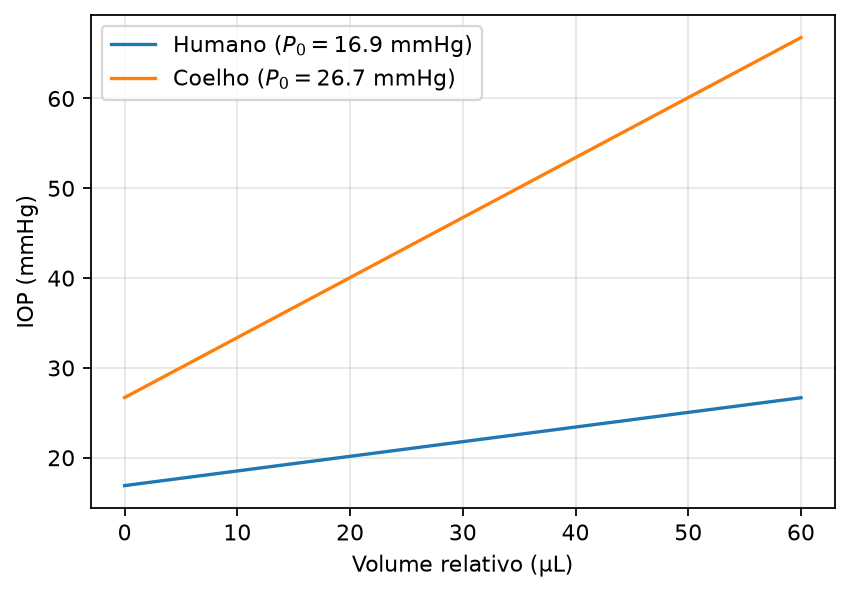
\includegraphics[width=0.55\textwidth]{Figuras/fig1_linear_comparativo.png}
\caption{Forma linear de $P(V)$, humano ($P_0=\SI{16{,}9}{\milli\meter Hg}$) e coelho anestesiado ($P_0=\SI{26{,}7}{\milli\meter Hg}$), cada um no seu próprio ponto de equilíbrio fisiológico (Seção~\ref{sec:producao_trabecular}). É a única forma usada para o coelho neste relatório, com o mesmo $E=\SI{3{,}0}{\mega\pascal}$ (estimativa de trabalho, Tabela~\ref{tab:E_esclera}). Para $\SI{50}{\micro\liter}$, o pico linear previsto para o coelho fica em torno de $\SI{60}{\milli\meter Hg}$, ordem de grandeza sem confronto clínico neste documento.}
\label{fig:linear_comparativo}
\end{figure}
 
A segunda forma é a lei de Friedenwald, que descreve o comportamento observado em olhos reais de maneira exponencial \citep{friedenwald1937},
 
\begin{equation}
\log_{10} P = \log_{10} P_0 + K_f\,(V-V_0),
\label{eq:friedenwald}
\end{equation}

onde $K_f$ é o coeficiente de rigidez ocular de Friedenwald e $V_0$ é o volume de referência no qual $P=P_0$ (neste relatório, $V_0=0$ no estado basal adotado antes da injeção). A curva $P(V)$ do globo reflete a parede corneoescleral \citep{ethier2004biomech}. Com $E=3{,}0$ MPa, a forma linear ($K=0{,}163$ mmHg/µL) fica $\approx24\%$ abaixo da curva de Friedenwald em 50 µL. Em olhos humanos vivos, o coeficiente foi medido por injeção manométrica direta de volume, com $K_f=0{,}0126\ \unit{\per\micro\liter}$ \citep{pallikaris2005}, e estimado por pneumotonometria diferencial, que não injeta volume, com $K_f=0{,}0252\ \unit{\per\micro\liter}$ em olhos normais \citep{kazemi2021}. Este último estudo também encontra rigidez menor em olhos com glaucoma ($K_f=0{,}0218\ \unit{\per\micro\liter}$).
 
Os valores de $K_f$ discutidos acima divergem, e a diferença de mecanismo e de faixa de medida é a explicação mais plausível, resumida na Tabela~\ref{tab:kf_comparacao}. 
 
\begin{table}[htbp]
\centering
\caption{Os três valores de $K_f$ usados ou discutidos neste relatório, com o mecanismo de medição e a particularidade que explica a divergência entre eles.}
\label{tab:kf_comparacao}
\small
\begin{tabular}{p{2.4cm}p{1.5cm}p{4.4cm}p{5.3cm}}
\toprule
Fonte & $K_f$ & O que mede & Particularidade \\
\midrule
\citet{pallikaris2005} &
$0{,}0126$ &
Injeção manométrica direta na câmara anterior, $79$ olhos de cirurgia de catarata, perturbação grande (até $200\ \unit{\micro\liter}$, em passos de $4{,}5\ \unit{\micro\liter}$) &
Mecanismo mais parecido com o deste relatório, mas calibrado só entre $10$ e $\SI{35}{\milli\meter Hg}$ de IOP, partindo de $\SI{10}{\milli\meter Hg}$. Extrapolar para picos acima de $\SI{50}{\milli\meter Hg}$ sai da faixa validada. \\
\addlinespace
\citet{kazemi2021} &
$0{,}0252$ normal\newline $0{,}0218$ glaucoma &
Pneumotonometria diferencial (IOP medida com e sem um peso de $10\ \unit{\gram}$ na ponteira, decúbito dorsal). Diferença de leitura convertida em $\Delta V$ equivalente por tabela de calibração, sem injeção real &
Perturbação mecânica externa minúscula, não injeção de volume. Mede rigidez de repouso, não resposta a bolus grande. Compara diretamente normal vs. glaucoma no mesmo protocolo. O intervalo de confiança de $95\%$ do grupo normal vai de $0{,}0230$ a $0{,}0280$. \\

\addlinespace
Recalibrado (este relatório) &
$0{,}00504$--$0{,}00656$\newline ($0{,}00581$ adotado) &
Não é medido. É a inversão algébrica da lei de Friedenwald usando o pico do \citet{knecht2009} como alvo, a partir do basal $P_0=\SI{16{,}9}{\milli\meter Hg}$ adotado neste relatório (Seção~\ref{sec:producao_trabecular}). Os limites vêm dos picos precisos relatados ($30{,}19$ e $35{,}97$ mmHg). O valor adotado vem do alvo $P=\SI{33}{\milli\meter Hg}$ (centro arredondado do intervalo $30$--$36$ relatado pelo estudo) &
Único calibrado exatamente no cenário de interesse (mesmo volume, mesma via, pico agudo real), mas por construção matemática, não por manometria, e depende de um único estudo. Trata-se de um $K_f$ efetivo de ajuste ($2$--$4\times$ abaixo dos $K_f$ manométricos ou pneumotonométricos acima), sensível ao basal assumido. Com $P_0=\SI{14}{\milli\meter Hg}$ e o mesmo pico-alvo, $K_f\approx0{,}00745$ ($+28\%$). Com $P_0=\SI{22}{\milli\meter Hg}$, $K_f\approx0{,}00352$ ($-39\%$). O Knecht não reporta basal único para a inversão. \\
\bottomrule
\end{tabular}
\end{table}
 
A Figura~\ref{fig:humano_pv} compara a forma linear de casca com três leis de Friedenwald para $P_0=\SI{16{,}9}{\milli\meter Hg}$, usando $K_f$ de \citet{pallikaris2005}, de \citet{kazemi2021} e a recalibração contra o pico de IVI de \citet{knecht2009} (Tabela~\ref{tab:kf_comparacao}). Só a recalibrada ($K_f=0{,}00581$ µL$^{-1}$) entra na dinâmica do WP0. Em $\SI{50}{\micro\liter}$ ela dá $\approx\SI{33}{\milli\meter Hg}$, a mais branda entre as candidatas. A linear prevê $\SI{25}{\milli\meter Hg}$ e fica abaixo do alvo de calibração. Com o $K_f$ de \citet{pallikaris2005} na forma $P=P_0\,10^{K_f V}$ (Equação~\ref{eq:friedenwald} em escala log), a projeção sobe para $\SI{72{,}1}{\milli\meter Hg}$. Se, em vez de multiplicar $P_0$, soma-se a ele o $\Delta P$ que \citet{pallikaris2005} mediu na câmara anterior a partir de $\SI{10}{\milli\meter Hg}$ ($P=P_0+\Delta P_{\text{art}}$), o pico cai para $\approx\SI{49{,}6}{\milli\meter Hg}$. A curva de \citet{kazemi2021} serve só de referência no painel e extrapola para valores não plausíveis em $\SI{50}{\micro\liter}$ (Seção~\ref{sec:camada2_pico}).
 
\begin{figure}[htbp]
\centering
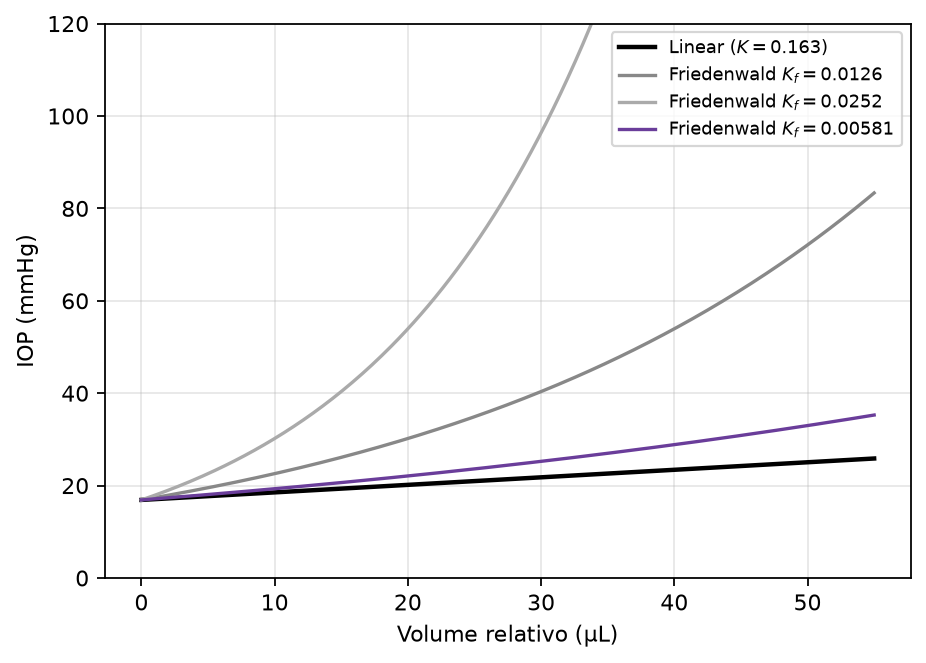
\includegraphics[width=0.62\textwidth]{Figuras/fig2_humano_friedenwald.png}
\caption{Forma linear e Friedenwald para humano com $P_0=\SI{16{,}9}{\milli\meter Hg}$. Curvas com $K_f$ de \citet{pallikaris2005}, \citet{kazemi2021} e recalibração contra o pico de \citet{knecht2009} ($K_f=\SI{0{,}00581}{\per\micro\liter}$, $\SI{33}{\milli\meter Hg}$ em $\SI{50}{\micro\liter}$). Em $\SI{50}{\micro\liter}$, \citet{pallikaris2005} dá $\SI{72{,}1}{\milli\meter Hg}$ com $P=P_0\,10^{K_f V}$ e $\approx\SI{49{,}6}{\milli\meter Hg}$ com $P=P_0+\Delta P_{\text{art}}$. \citet{kazemi2021} extrapola para $\SI{307{,}5}{\milli\meter Hg}$. Eixo cortado em $\SI{120}{\milli\meter Hg}$.}
\label{fig:humano_pv}
\end{figure}
 
\subsection{Injeção Intravítrea}
 
A injeção intravítrea é modelada como uma rampa de vazão constante durante um intervalo curto de tempo,
 
\begin{equation}
Q_{\text{ivi}}(t) =
\begin{cases}
\dfrac{V_{\text{inj}}}{\Delta t_{\text{inj}}}, & t_0 \le t \le t_0+\Delta t_{\text{inj}}, \\[6pt]
0, & \text{caso contrário},
\end{cases}
\label{eq:ivi}
\end{equation}
 
onde $V_{\text{inj}}$ é o volume total injetado e $\Delta t_{\text{inj}}$ é a duração da injeção. Adota-se $\Delta t_{\text{inj}}=\SI{6}{\second}$ (premissa do modelo). Essa é a única fonte de entrada de volume além da produção fisiológica, e é ela que provoca o pico agudo de pressão. O trabalho de \citet{ruffini2024} modela a expansão e a deflação do globo após a injeção com uma estrutura de balanço semelhante, mas sem detalhar a injeção como uma rampa de duração finita.
 
A justificativa para tratar essa etapa como quase estática, sem necessidade de resolver o escoamento do fluido dentro do olho, vem da comparação entre duas escalas de tempo. A velocidade com que uma variação de pressão se propaga através da parede elástica do globo é estimada pela relação de Moens e Korteweg \citep{fung1997},
 
\begin{equation}
c_{\text{MK}} = \sqrt{\frac{E\,t}{2\,\rho\,R}},
\label{eq:moens_korteweg}
\end{equation}
 
onde $\rho$ é a densidade do fluido. A fórmula completa de Korteweg inclui a compressibilidade do líquido, $c=\sqrt{(K_{\mathrm{B}}/\rho)\,/\,[1+K_{\mathrm{B}} D/(E t)]}$, em que $K_{\mathrm{B}}=\SI{2{,}2}{\giga\pascal}$ é o módulo de compressibilidade do líquido e $D$ o diâmetro. Aqui $K_{\mathrm{B}} D/(Et)\approx3{,}5\times10^{4}\gg1$, de modo que a parede complacente é o fator limitante da onda e a Equação~\ref{eq:moens_korteweg} é uma boa aproximação. A velocidade do som no líquido ($\approx\SI{1500}{\meter\per\second}$) só seria relevante com parede rígida. Usando $E=\SI{3{,}0}{\mega\pascal}$, com $t=\SI{0{,}5}{\milli\meter}$, $\rho=\SI{1000}{\kilo\gram\per\meter\cubed}$ e $R=\SI{12}{\milli\meter}$, o resultado é $c_{\text{MK}}\approx\SI{7{,}9}{\meter\per\second}$. Calculado para um diâmetro total do globo de $\SI{24}{\milli\meter}$, a onda atravessa o globo em $\approx\SI{3}{\milli\second}$, muito inferior a $\Delta t_{\text{inj}}$. Isso justifica que a parede acompanhe quase instantaneamente o bolus, assumindo um único compartimento pressurizado.
 
\subsection{Refluxo pelo trajeto da agulha}
 
Após a retirada da agulha, uma pequena quantidade de líquido pode escapar pelo canal deixado na esclera. Esse fenômeno é modelado não como uma vazão contínua, como a injeção, mas como uma perda de volume instantânea, aplicada no exato momento em que a injeção termina,
 
\begin{equation}
V(t_0+\Delta t_{\text{inj}}^+) = V(t_0+\Delta t_{\text{inj}}^-) - \Delta V_{\text{refluxo}}.
\label{eq:refluxo}
\end{equation}
 
Essa escolha de modelagem reflete uma observação experimental em olhos suínos \citep{brodie2014}, com refluxo em jato no instante da retirada da agulha, volume médio $\approx1{,}19$ µL, sem vazamento prolongado. O mesmo $\Delta V_{\text{refluxo}}$ é aplicado ao humano como ordem de grandeza. A composição do refluxo, majoritariamente vítreo \citep{brodie2014}, não entra no balanço, que depende só do volume que deixa a cavidade.
 
No presente estudo, com $P_0=\SI{16{,}9}{\milli\meter Hg}$, na forma linear ($K=0{,}163$), o pico de $\SI{25{,}0}{\milli\meter Hg}$ cai para $\SI{24{,}8}{\milli\meter Hg}$ logo após o refluxo, uma queda de $\SI{0{,}19}{\milli\meter Hg}$. Na forma Friedenwald recalibrada ($K_f=0{,}00581$, pico de $\SI{32{,}9}{\milli\meter Hg}$), a queda é de $\SI{0{,}52}{\milli\meter Hg}$ (de $32{,}90$ para $\SI{32{,}38}{\milli\meter Hg}$), $2{,}7$ vezes maior em valor absoluto. Ambas disponíveis na Figura~\ref{fig:refluxo_humano}.

Mesmo o maior dos dois valores ($0{,}52\ \unit{\milli\meter Hg}$, Friedenwald recalibrada) está abaixo da resolução prática da tonometria de aplanação de Goldmann, em geral lida em incrementos de $\SI{1}{\milli\meter Hg}$ \citep{goldmannschmidt1957}.

\FloatBarrier
\begin{figure}[htbp]
\centering
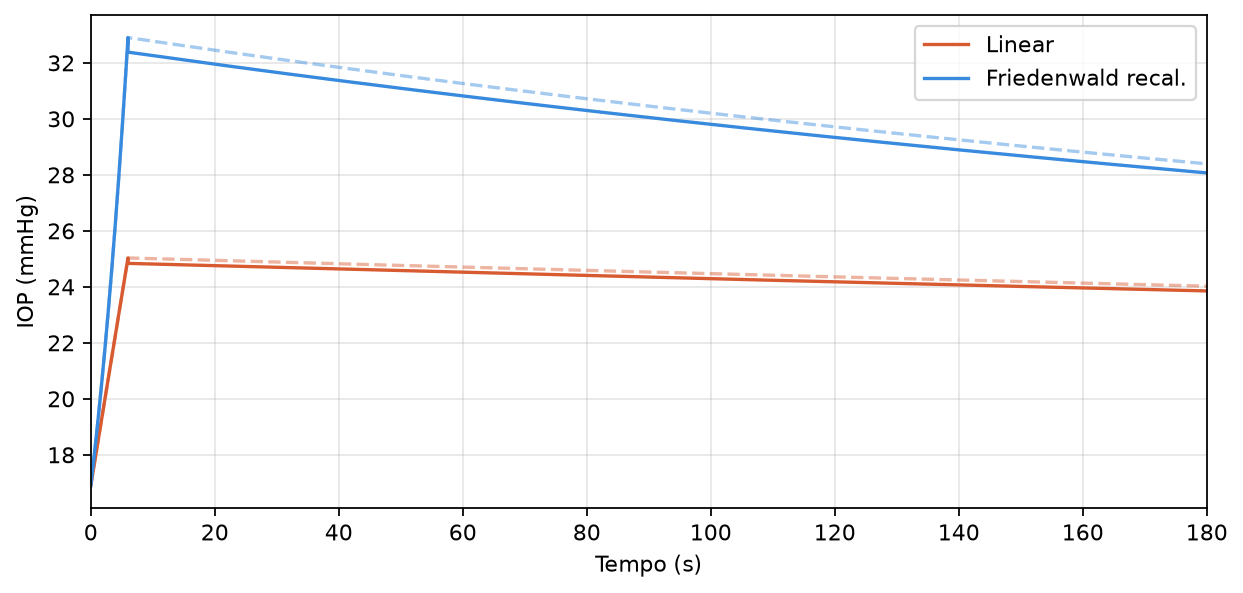
\includegraphics[width=0.95\textwidth]{Figuras/fig_refluxo_humano.png}
\caption{Efeito do refluxo sobre a curva de IOP, humano ($P_0=\SI{16{,}9}{\milli\meter Hg}$), zoom nos primeiros $3$ minutos, linear e Friedenwald recalibrada (linha contínua com refluxo, tracejada sem refluxo). A queda logo após o refluxo é maior em Friedenwald porque a lei exponencial amplifica a queda proporcionalmente ao próprio valor da pressão. Nas duas formas, as curvas convergem novamente ao longo do decaimento, porque o refluxo desloca o ponto de partida, não a dinâmica de retorno ao basal.}
\label{fig:refluxo_humano}
\end{figure}

\subsection{Paracentese}
 
A paracentese é modelada como um escoamento governado pela lei de Poiseuille através de uma agulha, durante um intervalo de tempo,
 
\begin{equation}
Q_{\text{par}}(t,P) =
\begin{cases}
\dfrac{(P-P_{\text{atm}})}{R_{\text{par}}}, & t_{\text{par}} \le t \le t_{\text{par}}+\Delta t_{\text{par}}, \\[6pt]
0, & \text{caso contrário},
\end{cases}
\label{eq:par_vazao}
\end{equation}
 
onde $R_{\text{par}}$ é a resistência hidráulica do trajeto de drenagem, calculada a partir do raio interno e do comprimento da agulha utilizada \citep{white2011},
 
\begin{equation}
R_{\text{par}} = \frac{8\,\mu\,L}{\pi\,a^4}
\label{eq:par_resistencia}
\end{equation}
 
em que $\mu$ é a viscosidade do humor aquoso, $L$ é o comprimento do trajeto percorrido pelo fluido e $a$ é o raio interno \citep{white2011}. Diferentemente do refluxo, a paracentese é tratada como um processo contínuo dentro da sua janela de atuação, pois o instrumento permanece inserido durante a drenagem, e o fluido efetivamente percorre todo o comprimento do seu canal interno.

Os parâmetros usados na Equação~\ref{eq:par_resistencia} incluem raio interno $a=\SI{0{,}0795}{\milli\meter}$ (diâmetro interno $\SI{0{,}159}{\milli\meter}$, agulha calibre $30$G) \citep{henein2019}, comprimento do trajeto $L=\SI{13}{\milli\meter}$ \citep{aiello2004, doshi2011, henein2019} e viscosidade do humor aquoso $\mu=\SI{0{,}75}{\milli\pascal\second}$ (próxima à da água a $\SI{37}{\celsius}$) \citep{heys2001, dvoriashyna2019, repetto2015}, resultando em $R_{\text{par}}=6{,}2\times10^{11}\ \unit{\pascal\second\per\meter\cubed}$ segundo a lei de Hagen--Poiseuille \citep{ocularfluiddynamics, peng2025}.
 
A duração da janela, $\Delta t_{\text{par}}$, não possui registro na literatura e, por isso, é calculada como o tempo necessário para drenar o volume retirado, adotado igual ao volume injetado, $\SI{50}{\micro\liter}$ \citep{changchung2007, soheilian2017}, e a paracentese é encerrada quando esse volume é atingido. Esse tempo não é uma constante da agulha, porque depende da pressão em que a drenagem começa. Como a vazão é proporcional à pressão, e a pressão diminui à medida que o volume escoa, a drenagem desacelera ao longo do processo.
 
Integrando numericamente a Equação~\ref{eq:par_vazao} para a retirada de $\SI{50}{\micro\liter}$, o resultado depende do ponto de partida. A partir da pressão basal ($\SI{16{,}9}{\milli\meter Hg}$), a drenagem leva $\Delta t_{\text{par}}=\SI{18{,}8}{\second}$ na forma linear e $\SI{19{,}6}{\second}$ na recalibrada. A partir da pressão já elevada pela injeção, leva de $\SI{10{,}5}{\second}$ a $\SI{11{,}8}{\second}$, porque a vazão inicial é maior. Como verificação de ordem de grandeza, mesmo que a pressão permanecesse em $\SI{16{,}9}{\milli\meter Hg}$ durante toda a drenagem, a vazão inicial de $\SI{3{,}6}{\micro\liter\per\second}$ exigiria $\SI{13{,}8}{\second}$, de modo que nenhuma duração inferior a esse valor é compatível com a retirada de $\SI{50}{\micro\liter}$ a partir do basal. 

O escoamento na agulha é laminar e desenvolvido, com $Q\approx\SI{3{,}6}{\micro\liter\per\second}$, o número de Reynolds é $\approx39$ e o comprimento de entrada ($\approx0{,}06\,Re\,d$) é $\approx\SI{0{,}4}{\milli\meter}$, pequeno frente a $L=\SI{13}{\milli\meter}$, o que valida a lei de Poiseuille.
 
Este relatório simula três instantes distintos de início da paracentese em relação à injeção, correspondendo a três estratégias clínicas diferentes, descritas a seguir.
 
\begin{itemize}
\item Profilática ($t=-\SI{30}{\second}$ antes da injeção): realizada de $t=-\SI{30}{\second}$ até $t=-\SI{11{,}2}{\second}$ na forma linear ($\Delta t_{\text{par}}=\SI{18{,}8}{\second}$) ou até $t=-\SI{10{,}4}{\second}$ na recalibrada ($\Delta t_{\text{par}}=\SI{19{,}6}{\second}$), terminando, portanto, entre $\SI{10{,}4}{\second}$ e $\SI{11{,}2}{\second}$ antes do início da injeção. É o desenho usado por protocolos como o de \citet{soheilian2017}, e é modelada aqui como três fases sequenciais e não sobrepostas (paracentese, intervalo livre residual, depois injeção).
\item Reativa ($t=+\SI{30}{\second}$ após a injeção): realizada assim que se percebe uma elevação de pressão, mas o pico agudo, que se forma em segundos, já ocorreu. A drenagem começa em pressão elevada e leva $\SI{11{,}5}{\second}$ na forma linear e $\SI{10{,}5}{\second}$ na recalibrada.
\item Tardia ($t=+\SI{2}{\minute}$ após a injeção): realizada bem depois que o pico já se formou por completo, seguindo prática relatada por oftalmologistas que preferem confirmar a elevação antes de intervir. A drenagem leva $\SI{11{,}8}{\second}$ na forma linear e $\SI{11{,}3}{\second}$ na recalibrada.
\end{itemize}
 
Como a paracentese profilática termina antes de a injeção começar e o pico se forma durante $\Delta t_{\text{inj}}$, apenas a profilática consegue reduzir o próprio pico. A reativa e a tardia começam depois que o pico já aconteceu.
 
De acordo com os resultados obtidos por \citet{soheilian2017}, um grupo sem paracentese, com IOP basal de $14{,}2\pm2{,}0\ \unit{\milli\meter Hg}$, sobe para $40{,}6\ \unit{\milli\meter Hg}$ aos dois minutos (aumento de $+26{,}4\pm5{,}7$), caindo para $20{,}7\ \unit{\milli\meter Hg}$ aos trinta minutos. Um grupo com paracentese profilática, com IOP basal de $13{,}8\pm2{,}3\ \unit{\milli\meter Hg}$, vai para apenas $12{,}5\ \unit{\milli\meter Hg}$ aos dois minutos (variação de $-1{,}3\pm2{,}4$) e $10{,}6\ \unit{\milli\meter Hg}$ aos trinta minutos (variação de $-3{,}2\pm1{,}8$).
 
A Figura~\ref{fig:paracentese_humano} mostra que, na forma recalibrada, o pico cai de $\SI{32{,}9}{\milli\meter Hg}$ (sem intervenção) para $\SI{17{,}1}{\milli\meter Hg}$ na profilática, uma redução de $48\%$. Na forma linear, o pico cai de $\SI{25{,}0}{\milli\meter Hg}$ para $\SI{17{,}1}{\milli\meter Hg}$, uma redução de $32\%$, menor em valor absoluto porque o pico linear já é pequeno mesmo sem intervenção. Como o volume retirado é igual ao injetado, a profilática anula o efeito da injeção, a drenagem leva a pressão a $\SI{8{,}7}{\milli\meter Hg}$ na forma recalibrada e a $\SI{8{,}8}{\milli\meter Hg}$ na linear, e a injeção a traz de volta ao redor do basal, sem ultrapassá-lo. Reativa e tardia não alteram o pico. Na forma recalibrada, a pressão mínima é $\SI{16{,}2}{\milli\meter Hg}$ (reativa, $+30$ s) e $\SI{15{,}0}{\milli\meter Hg}$ (tardia, $+2$ min), mais baixa quanto mais tarde a intervenção, porque, quanto mais tempo passa, mais do volume injetado já saiu pelas vias fisiológicas, e a retirada de $\SI{50}{\micro\liter}$ passa a ultrapassar o excesso. Nas estratégias reativa e tardia, o retorno final ao basal ocorre por produção fisiológica, muito mais lento do que a queda induzida pela paracentese em si.
 
\begin{figure}[htbp]
\centering
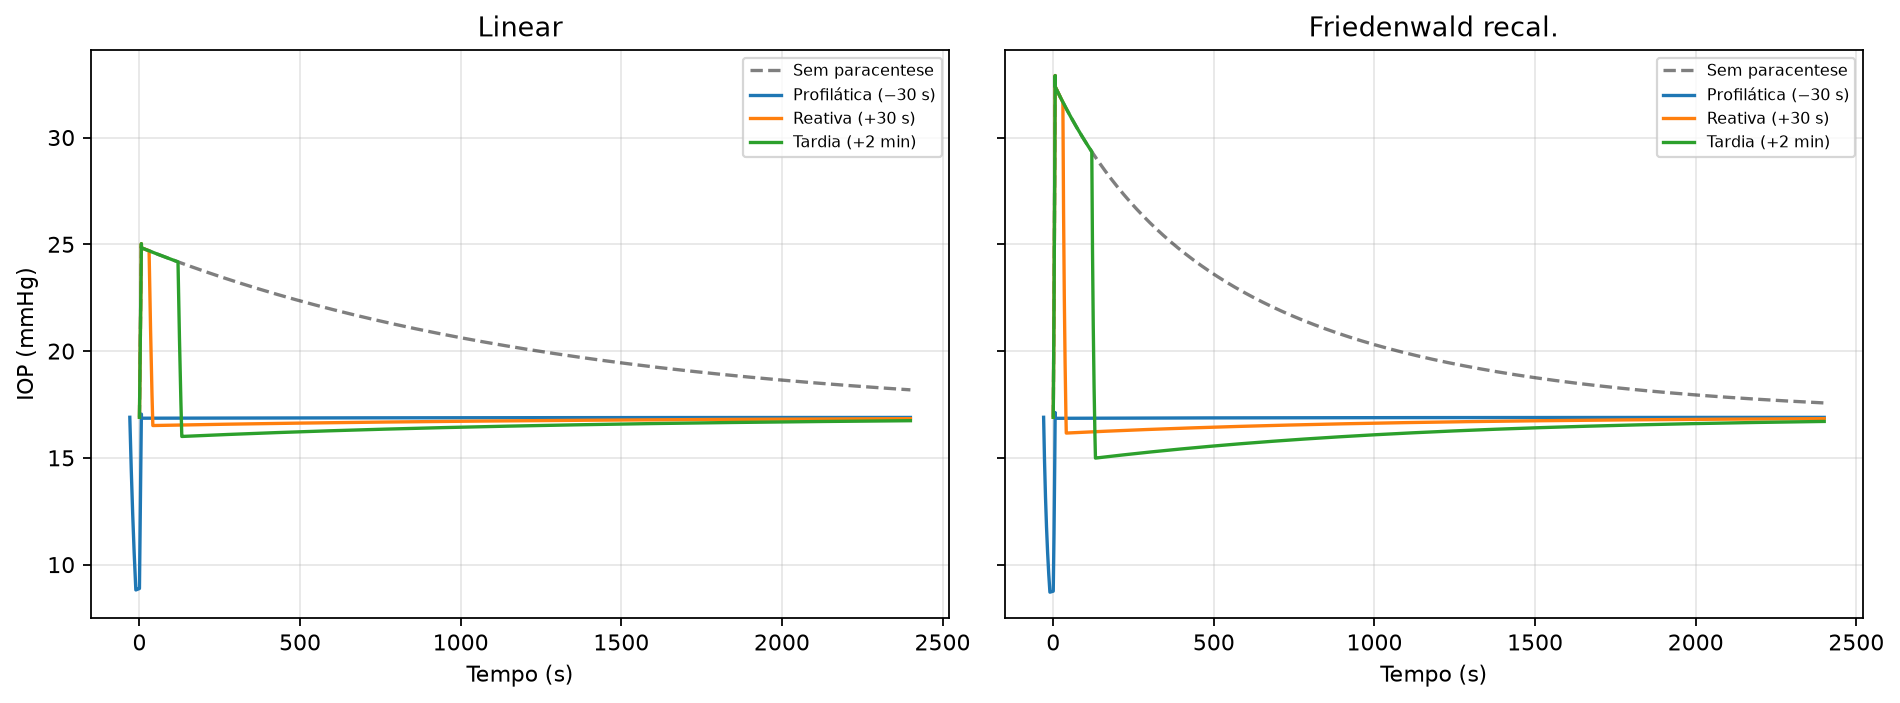
\includegraphics[width=0.98\textwidth]{Figuras/fig_paracentese_3cenarios.png}
\caption{Efeito da paracentese sobre a curva de IOP em três estratégias (linhas: profilática $t=-30$s, reativa $t=+30$s, tardia $t=+2$min), com a drenagem encerrada ao atingir $\SI{50}{\micro\liter}$, contra as duas formas de $P(V)$ efetivamente usadas neste relatório.}
\label{fig:paracentese_humano}
\end{figure}
 
\subsection{Produção trabecular e uveoescleral}
\label{sec:producao_trabecular}
 
O escoamento do humor aquoso, responsável por trazer a pressão de volta ao valor basal após a injeção, ocorre por duas vias distintas. A via trabecular é a via convencional descrita pela relação de Goldmann \citep{goel2010,brubaker2004},
 
\begin{equation}
Q_{TM}(P) = C_{\text{out}}\,(P-P_{ev}),
\label{eq:trabecular}
\end{equation}
 
onde $C_{\text{out}}$ é a facilidade de escoamento trabecular e $P_{ev}$ é a pressão venosa episcleral. Na implementação numérica, $Q_{TM}$ não é truncado em zero quando $P<P_{ev}$. Na paracentese profilática, a forma recalibrada atinge $\approx\SI{8{,}7}{\milli\meter Hg}<P_{ev}=\SI{10}{\milli\meter Hg}$. O influxo trabecular resultante é de $\approx\SI{0{,}36}{\micro\liter\per\minute}$ e altera a IOP em menos de $\SI{0{,}02}{\milli\meter Hg}$.
 
A via uveoescleral, por sua vez, drena uma parte do humor aquoso de maneira quase independente da IOP, sendo descrita apenas como uma fração da produção total,
 
\begin{equation}
Q_{uv} = f_{uv}\,Q_{\text{prod}}.
\label{eq:uveoscleral}
\end{equation}
 
A fração $f_{uv}$ varia entre espécies, sendo pequena em coelhos e gatos, devido ao pouco desenvolvimento do músculo ciliar nessas espécies, e substancialmente maior em primatas e humanos \citep{alm2009}. A Tabela~\ref{tab:especies} reúne os valores experimentais disponíveis nas espécies discutidas neste relatório.
 
\begin{table}[htbp]
\centering
\caption{Parâmetros de escoamento fisiológico por espécie, com fonte.}
\label{tab:especies}
\begin{tabular}{lp{4.2cm}p{4.2cm}}
\toprule
 & \centering Humano & \centering\arraybackslash Coelho (anestesiado) \\
\midrule
$Q_{\text{prod}}$ (\unit{\micro\liter\per\minute}) & $2{,}4\pm0{,}6$ \citep{goel2010} & $3{,}06\pm0{,}6$ \citep{kiel2011ciliary} \\
$C_{\text{out}}$ (\unit{\micro\liter\per\minute\per\milli\meter Hg}) & $0{,}28$ \citep{goel2010} & $0{,}26\pm0{,}07$ \citep{fourman1989outflow} \\
$P_{ev}$ (\unit{\milli\meter Hg}) & $10$ \citep{ethier2004biomech} & $15$--$16$ \citep{kiel2015evp} \\
$f_{uv}$ (\% do total) & $\approx 20$ \citep{goel2010,alm2009} & $3$--$8$ \citep{alm2009} \\
\bottomrule
\end{tabular}
\end{table}
 
Fixa-se $P_0=\SI{16{,}9}{\milli\meter Hg}$. Com $Q_{\text{prod}}=\SI{2{,}4}{\micro\liter\per\minute}$ e os demais valores da Tabela~\ref{tab:especies}, o repouso seria $\SI{16{,}86}{\milli\meter Hg}$. Para fechar $\SI{16{,}9}{\milli\meter Hg}$ com $dV/dt=0$ sem injeção, adota-se $Q_{\text{prod}}=\SI{2{,}415}{\micro\liter\per\minute}$, dentro de $2{,}4\pm0{,}6$. O basal vem do equilíbrio $P_0=P_{ev}+Q_{\text{prod}}(1-f_{uv})/C_{\text{out}}$.
 
Aplicando o mesmo cálculo aos parâmetros do coelho anestesiado ($Q_{\text{prod}}=3{,}06$, $C_{\text{out}}=0{,}26$, $f_{uv}=0{,}05$, $P_{ev}=15{,}5$, meio da faixa $15$--$16$), o resultado é $P_0=15{,}5+3{,}06\times0{,}95/0{,}26\approx\SI{26{,}7}{\milli\meter Hg}$. Esse valor é consistente com a IOP basal de coelho anestesiado relatada entre $16{,}2$ e $\SI{33{,}2}{\milli\meter Hg}$ \citep{kiel2015evp}, contra apenas $7$--$\SI{16}{\milli\meter Hg}$ em coelho acordado. O valor de $C_{\text{out}}$ usado, medido em coelho não anestesiado, é o único disponível na literatura revisada. Não foi encontrada uma medição direta de $C_{\text{out}}$ sob anestesia geral.
 
Os dois termos do escoamento, trabecular e uveoescleral, são responsáveis pela recuperação do equilíbrio após o término da injeção. O quão rápido isso acontece está associado à constante de tempo
 
\begin{equation}
\tau = \frac{1}{C_{\text{out}}\,K},
\label{eq:tau}
\end{equation}
 
que resulta da linearização da equação de balanço em torno do estado de equilíbrio, e que determina o perfil de resposta do sistema. Para o coelho, que usa a forma linear, $K$ nessa fórmula é a mesma constante $K=0{,}668$ da Equação~\ref{eq:casca_fina}. Para o humano recalibrado, usa-se $K_{\text{local}}=dP/dV$ no basal, $K_{\text{local}}=\ln(10)\cdot K_f\cdot P_0=2{,}30\times0{,}00581\times16{,}9\approx\SI{0{,}226}{\milli\meter Hg\per\micro\liter}$, o que com $C_{\text{out}}=0{,}28$ dá $\tau=1/(0{,}28\times0{,}226)\approx\SI{15{,}8}{\minute}$.

A Figura~\ref{fig:decaimento} mostra a curva completa de retorno ao valor basal, para humano e coelho, com a constante de tempo de cada espécie ($\tau_{\text{humano}}=\SI{15{,}8}{\minute}$ no basal, $\tau_{\text{coelho}}=\SI{5{,}76}{\minute}$). No humano, a rigidez local da forma de Friedenwald cresce com a pressão, de modo que $\tau$ cai para $\SI{8{,}1}{\minute}$ no pico e a queda é mais rápida no início, aproximando-se de $\SI{15{,}8}{\minute}$ ao final. Com refluxo ligado, aos $10$ min dissipa-se cerca de $64\%$ do excesso pós-pico, aos $50$ min, $98\%$.
 
\begin{figure}[htbp]
\centering
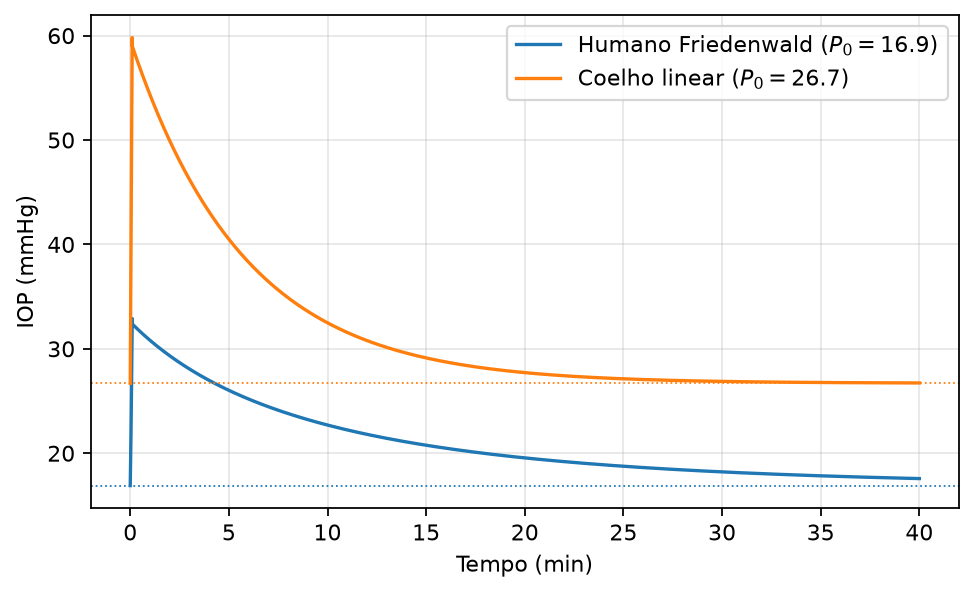
\includegraphics[width=0.65\textwidth]{Figuras/fig_decaimento.png}
\caption{Retorno ao basal após injeção de $\SI{50}{\micro\liter}$ via escoamento trabecular e uveoescleral combinados, humano ($P_0=\SI{16{,}9}{\milli\meter Hg}$) e coelho anestesiado ($P_0=\SI{26{,}7}{\milli\meter Hg}$). No basal, o $\tau$ do coelho ($\SI{5{,}76}{\minute}$) é $2{,}7$ vezes menor que o do humano ($\SI{15{,}8}{\minute}$).}
\label{fig:decaimento}
\end{figure}
 
\section{Verificação}
\label{sec:validacao}
 
\subsection{Parte 1 --- verificação numérica}
\label{sec:camada1_ruffini}

Antes de qualquer comparação com dado biológico, verifica-se se o solver resolve corretamente a equação diferencial. Para isso, utiliza-se o artigo de \citet{ruffini2024}, que também descreve um modelo 0D linear, com produção efetiva de $Q_{in}=2{,}2\ \unit{\micro\liter\per\minute}$, pressão episcleral de $P_{ev}=\SI{8}{\milli\meter Hg}$ e complacência ocular constante de $C=\SI{1}{\micro\liter\per\milli\meter Hg}$ (rigidez $K\approx0{,}05\ \unit{\per\micro\liter}$ medida por \citet{collins1980mathematical} na base natural, $\ln P=\ln P_0+K(V-V_0)$, equivalente a $K_f\approx0{,}05/\ln(10)\approx0{,}022\ \unit{\per\micro\liter}$ na forma em $\log_{10}$ da Equação~\ref{eq:friedenwald}), obtendo analiticamente uma constante de tempo de decaimento $\tau=\SI{3{,}18}{\minute}$ (valor arredondado do resumo). No protocolo de verificação deste relatório ($\SI{50}{\micro\liter}$ em $\SI{6}{\second}$, refluxo desligado, $f_{uv}=0$, $C_{\text{out}}=Q_{in}/(P_{\text{eq}}-P_{ev})$ com $P_{\text{eq}}=\SI{15}{\milli\meter Hg}$ de equilíbrio do teste), o valor analítico linearizado é $\tau_{\text{analítico}}=1/(C_{\text{out}}K)=\SI{3{,}18}{\minute}$. Um ajuste exponencial da curva simulada (baseline fixa em $\SI{15}{\milli\meter Hg}$, janela a partir do fim da injeção) reproduz esse $\tau$ com erro relativo de $\approx3{,}9\times10^{-7}$ (inferior a $10^{-6}$).
 
\subsection{Parte 2 --- pico agudo}
\label{sec:camada2_pico}
 
A Tabela~\ref{tab:literatura_master} reúne todas as fontes de literatura usadas neste relatório para calibrar ou validar a resposta de pressão pós-IVI, com espécie, volume de injeção, basal, pico e tipo de intervenção.
 
\begin{table}[htbp]
\centering
\caption{Fontes de literatura usadas na parametrização e validação deste relatório (todas em humanos).}
\label{tab:literatura_master}
\small
\resizebox{\textwidth}{!}{
\setlength{\tabcolsep}{5pt}
\begin{tabular}{p{2.4cm}p{1.9cm}p{1.7cm}p{1.7cm}p{6.5cm}}
\toprule
Fonte & IVI & Basal (mmHg) & Pico (mmHg) & Paracentese \\
\midrule
\citet{knecht2009} & $50$\,µL & --- & $30{,}2$--$36{,}0$ & Alvo de calibração de $K_f=0{,}00581$ (recalibrado) \\
\citet{soheilian2017}, Grupo A & $50$\,µL & $14{,}2$ & $40{,}6$ & Sem intervenção \\
\citet{soheilian2017}, Grupo B & $50$\,µL & $13{,}8$ & $12{,}5$ & Paracentese profilática \\
\citet{sharei2010} & $50$\,µL & $22{,}4$ & $47{,}9$ & Sem intervenção \\
\citet{hu2022conbercept} & $50$\,µL & $14{,}81$ & $26{,}80$ & Sem intervenção \\
\citet{papazoglou2026} & $50$\,µL & $13{,}98$ & $31{,}15$ (T2) & Sem intervenção \\
\citet{changchung2007} & $100$\,µL & $15{,}33$ & $46{,}7$ & Paracentese reativa/tardia (pós-paracentese $7{,}80$ mmHg). Volume diferente do padrão deste relatório \\
\bottomrule
\end{tabular}
}
 
\vspace{4pt}
\end{table}
\FloatBarrier
 
Nenhuma dessas fontes clínicas deriva ou mede $K_f$ diretamente. Os valores de $K_f$ usados neste relatório vêm exclusivamente da recalibração contra o Knecht (Seção~\ref{sec:balanco_geral}). As fontes clínicas de pico servem apenas para comparação externa do resultado final, não para parametrizar o modelo.

A Figura~\ref{fig:camada2} mostra as duas formas de $P(V)$ efetivamente usadas neste relatório junto com os pontos de pico medidos nos estudos sem intervenção.

\begin{figure}[htbp]
\centering
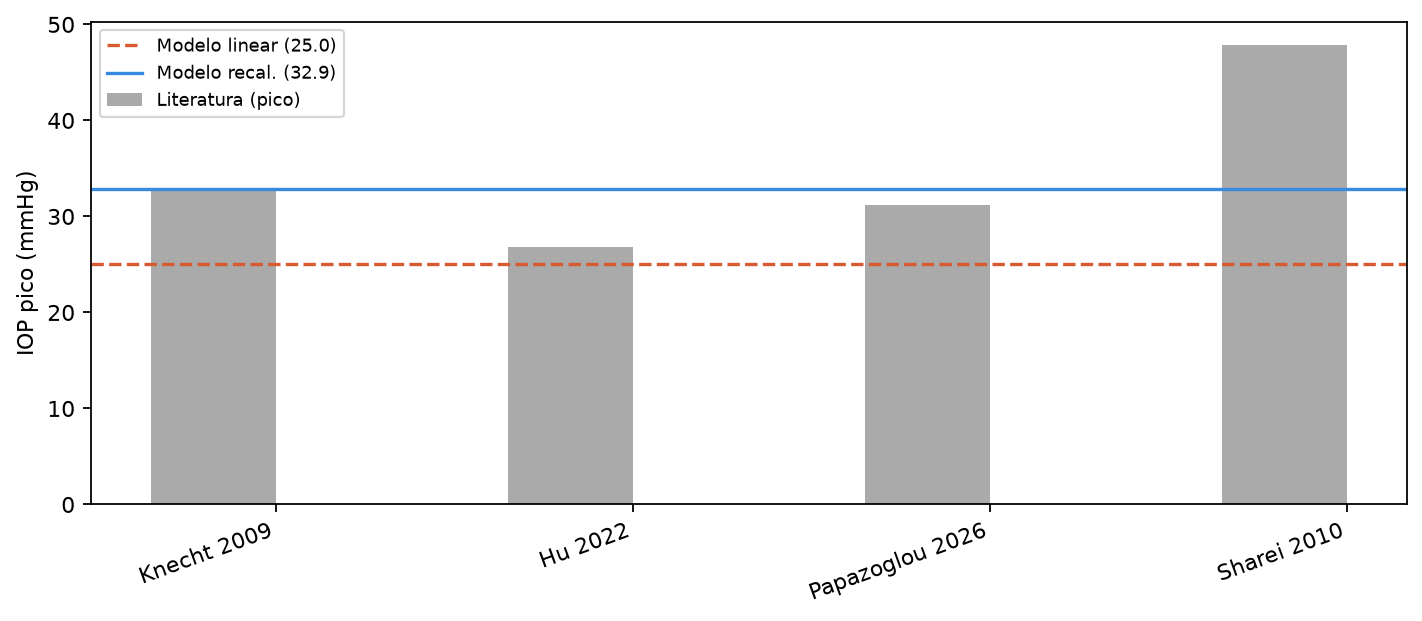
\includegraphics[width=0.85\textwidth]{Figuras/fig_camada2_picos.png}
\caption{Pico agudo pós-IVI para $\SI{50}{\micro\liter}$: as duas formas de $P(V)$ usadas neste relatório (sem paracentese, picos de $25{,}0$ e $\SI{32{,}9}{\milli\meter Hg}$ para linear e recalibrada, a partir de $P_0=\SI{16{,}9}{\milli\meter Hg}$) contra quatro estudos clínicos independentes (painel esquerdo: IOP absoluta; painel direito: aumento em relação ao basal de cada estudo). Os pontos clínicos correspondem a instantes de leitura diferentes (Tabela~\ref{tab:camada2_alinhada}).}
\label{fig:camada2}
\end{figure}
 
\citet{soheilian2017} relata, no grupo sem paracentese ($n=45$, bevacizumabe), IOP basal de $14{,}2\pm2{,}0\ \unit{\milli\meter Hg}$, subindo a $40{,}6\ \unit{\milli\meter Hg}$ aos dois minutos e caindo a $20{,}7\ \unit{\milli\meter Hg}$ aos trinta minutos.
 
\citet{sharei2010} relata, em $45$ olhos com ranibizumabe em posição supina, IOP basal de $22{,}4\pm5{,}5\ \unit{\milli\meter Hg}$ subindo a $47{,}9\pm15{,}1\ \unit{\milli\meter Hg}$ imediatamente após a injeção, com queda espontânea de $12{,}6$ aos três minutos e de $21$ aos dez minutos (pressões remanescentes $\approx35{,}3$ e $\approx26{,}9$ mmHg). O basal já elevado, característico da posição supina, explica o pico mais alto entre os estudos reunidos aqui.
 
\citet{hu2022conbercept} relata, em $40$ pacientes com Conbercept, IOP basal de $14{,}81\pm3{,}13\ \unit{\milli\meter Hg}$, subindo a $26{,}80\pm9{,}43\ \unit{\milli\meter Hg}$ aos dois minutos, $18{,}76\pm6{,}16$ aos dez minutos e $16{,}54\pm5{,}94$ aos trinta minutos.
 
\citet{papazoglou2026} mede IOP em três instantes. T1 é basal ($13{,}98\pm3{,}09\ \unit{\milli\meter Hg}$). T2 fica em $31{,}15\pm9{,}65\ \unit{\milli\meter Hg}$, com aquisição tipicamente iniciada em mediana $\approx\SI{7{,}5}{\minute}$ após a IVI. T3 fica dez minutos após T2 ($16{,}30\pm4{,}60\ \unit{\milli\meter Hg}$). Não é leitura imediata ao fim da agulha nem cota padronizada aos $2$ min.
 
\citet{knecht2009} relata pico medido em menos de um minuto de $35{,}97\pm8{,}13\ \unit{\milli\meter Hg}$ na técnica tunelizada e $30{,}19\pm12{,}14\ \unit{\milli\meter Hg}$ na técnica reta, mais convencional.

Os basais dos estudos diferem ($13{,}8$ a $\SI{22{,}4}{\milli\meter Hg}$), de modo que a comparação exige alinhar o instante de leitura. A Tabela~\ref{tab:camada2_alinhada} confronta, nesse instante, o aumento observado com o do modelo de referência (Friedenwald recalibrada, refluxo ligado, $P_0=\SI{16{,}9}{\milli\meter Hg}$).

\begin{table}[htbp]
\centering
\caption{Comparação alinhada no tempo: aumento de IOP ($\Delta P$) observado vs.\ modelo de referência.}
\label{tab:camada2_alinhada}
\small
\begin{tabular}{llrrr}
\toprule
Estudo & Instante & Observado & Modelo & Razão \\
\midrule
\citet{sharei2010} & imediato ($6$ s) & $+25{,}5$ & $+16{,}0$ & $1{,}6$ \\
\citet{soheilian2017} & $2$ min & $+26{,}4$ & $+12{,}4$ & $2{,}1$ \\
\citet{hu2022conbercept} & $2$ min & $+12{,}0$ & $+12{,}4$ & $1{,}0$ \\
\citet{papazoglou2026}, T2 & $\approx7{,}5$ min & $+17{,}2$ & $+7{,}2$ & $2{,}4$ \\
\bottomrule
\end{tabular}
\end{table}

O modelo subestima três dos quatro estudos em $1{,}6$ a $2{,}4\times$ e só concorda com \citet{hu2022conbercept}. Esse estudo reporta o menor aumento da Tabela~\ref{tab:camada2_alinhada} ($+12{,}0$ mmHg), de modo que a concordância pode ser coincidência com o extremo inferior da faixa clínica, e não acerto nos picos mais altos. O modelo reproduz, na prática, o limite inferior observado e subestima os demais. A forma linear ($K=0{,}163$ mmHg/µL) prevê, nos mesmos instantes, $+8{,}1$ mmHg ($6$ s) e $+7{,}3$ mmHg ($2$ min), ainda mais abaixo dos observados.

\subsection{Velocidade de retorno}
 
A terceira etapa testa não o pico, mas a velocidade com que a pressão volta ao normal depois dele. Para isso, \citet{lobue2023} mediram a IOP de $617$ pacientes a cada $10$ minutos após injeções de $\SI{0{,}05}{\milli\liter}$ e consideraram que o paciente havia retornado ao basal quando a IOP ficava a menos de $\SI{4}{\milli\meter Hg}$ do seu próprio valor pré-injeção. Isso ocorreu em $85\%$ dos pacientes aos $30$ minutos e em $98\%$ aos $50$ minutos. Na forma recalibrada, o olho do modelo atinge esse critério em $\SI{14{,}6}{\minute}$, antes dos $30$ minutos do percentil de $85\%$. O aumento médio observado aos $10$ minutos foi de $9\pm10$ mmHg e o modelo prevê $\SI{5{,}8}{\milli\meter Hg}$.
 
\subsection{Efeito da paracentese}
\label{sec:camada4}

Compara-se o efeito da paracentese contra três fontes da literatura. As três medem esse efeito da mesma forma, como a diferença de IOP entre um grupo com paracentese e um grupo sem, no mesmo instante.
 
\citet{soheilian2017} é a comparação mais direta, porque usa exatamente o volume de injeção deste relatório e divide a pesquisa em dois grupos, sem paracentese (Grupo A, pico de $40{,}6\ \unit{\milli\meter Hg}$ aos dois minutos) e com paracentese profilática (Grupo B, $12{,}5\ \unit{\milli\meter Hg}$ no mesmo instante). A diferença real entre os grupos é de $-28{,}1\ \unit{\milli\meter Hg}$ aos dois minutos e $-10{,}1\ \unit{\milli\meter Hg}$ aos trinta minutos. O cenário profilático simulado dá uma diferença de apenas $\SI{-12{,}5}{\milli\meter Hg}$ aos dois minutos e $\SI{-1{,}3}{\milli\meter Hg}$ aos trinta minutos. O modelo atual captura a direção do efeito, mas subestima a magnitude em ambos os instantes, por um fator de $2{,}3$ a $7{,}8\times$.

\citet{changchung2007} usa injeção de $\SI{100}{\micro\liter}$, o dobro do padrão deste relatório, o que impede comparar magnitudes de pico ou diferença aos dois minutos ($-38{,}9$ mmHg observados). Reporta-se apenas o contraste entre grupos aos quinze minutos, diferença real $-4{,}4$ mmHg contra $-4{,}8$ mmHg no cenário tardio simulado ($t_{\text{par}}=\SI{2}{\minute}$), ordem de grandeza semelhante.
 
\citet{zaman2025} agrega $13$ estudos clínicos com volumes e técnicas variadas, relatando diferenças médias de $-5{,}09\ \unit{\milli\meter Hg}$ aos dois minutos, $-2{,}37$ aos cinco minutos e $-1{,}54$ aos trinta minutos. Contra o mesmo cenário tardio simulado, o modelo dá $\SI{0{,}00}{\milli\meter Hg}$ aos dois minutos, $\SI{-10{,}8}{\milli\meter Hg}$ aos cinco minutos e $\SI{-1{,}7}{\milli\meter Hg}$ aos trinta minutos. O ajuste aos trinta minutos é bom ($-1{,}7$ contra $-1{,}5$), mas aos cinco minutos o modelo superestima o efeito em mais de $4\times$ ($-10{,}8$ contra $-2{,}4$).

Os três casos não mostram o mesmo padrão. Em \citet{soheilian2017}, com protocolo único e volume igual ao do modelo, o modelo subestima o efeito aos dois minutos, em boa parte porque a IOP prevista aos dois minutos sem intervenção ($\SI{29{,}3}{\milli\meter Hg}$) é menor que a observada no grupo A ($\SI{40{,}6}{\milli\meter Hg}$), embora o pico imediato simulado na forma recalibrada seja $\SI{32{,}9}{\milli\meter Hg}$. Esse desvio não se corrige variando $K_f$. Com o basal do próprio estudo ($14{,}2$ mmHg) e sem refluxo, a IOP simulada aos $2$ min vai de $\approx21$ a $\approx38$ mmHg quando $K_f$ sobe de $0{,}0035$ a $0{,}0150$ µL$^{-1}$ (pico imediato de $\approx21$ a $\approx78$ mmHg) e satura abaixo dos $40{,}6$ mmHg observados. Na faixa que cobre a incerteza do basal ($0{,}0035$ a $0{,}0075$), com $P_0=16{,}9$ mmHg, a IOP aos $2$ min chega a $\approx33{,}4$ mmHg e o pico imediato a $\approx40$ mmHg. Aos trinta minutos, o grupo B permanece abaixo do próprio basal ($-3{,}2$ mmHg), enquanto a profilática simulada já voltou ao basal.

Em \citet{changchung2007}, a diferença de $\SI{0{,}00}{\milli\meter Hg}$ aos dois minutos decorre do instante de início da paracentese simulada. Aos quinze minutos o modelo concorda com o observado ($-4{,}8$ contra $-4{,}4$).

Em \citet{zaman2025}, o modelo concorda aos trinta minutos ($-1{,}7$ contra $-1{,}5$) e superestima o efeito aos cinco ($-10{,}8$ contra $-2{,}4$). A paracentese simulada é um evento único e completo em $\SI{10{,}5}{\second}$ a $\SI{11{,}8}{\second}$, com queda abrupta logo depois. Quando o transitório já se dissipou, o que resta é dominado pela produção fisiológica.

\subsection{Limitações}
\label{sec:wp0_limitacoes}

Em comparação externa de pico (Seção~\ref{sec:camada2_pico}), o modelo subestima o aumento de IOP em três de quatro estudos ($1{,}6$ a $2{,}4\times$, Tabela~\ref{tab:camada2_alinhada}) e não deve ser usado para decisão clínica.

O modelo é zero-dimensional. Não resolve distribuição espacial de pressão nem deformação local dos tecidos. A geometria usa $R$ esférico e espessura média $t$, com $t$ de tecido não pressurizado \citep{vurgese2012}. A curva $P(V)$ global reflete a córnea e a esclera, sem resolver mecanismos microestruturais. Para o coelho, só entra a forma linear de casca, sem confronto de pico com estudos clínicos. O $P_0$ do coelho anestesiado depende de $C_{\text{out}}$ medido em animal acordado, por falta de dado direto sob anestesia. Comparar picos clínicos exige alinhar instante de leitura e basal (Tabela~\ref{tab:camada2_alinhada}). Vazamento pelo trajeto da agulha, sangue coroidal e viscoelasticidade ficam fora do 0D. Em \citet{lobue2023}, a faixa de aumento de IOP aos $10$ min ($-1$ a $+19$ mmHg, aprox.) limita o poder de discriminar o ajuste. Nenhum dos três confrontos de paracentese reproduz volume, tempo e população idênticos ao simulado (\citet{changchung2007} usa $100$ µL). A constante $K=0{,}163$ mmHg/µL da forma linear de casca levaria a outro $\tau$ humano se substituísse a complacência local da Friedenwald recalibrada na Equação~\ref{eq:tau}.

\newpage
\part{WP1 --- Modelagem Mecânica}

\section{WP1.1 --- Verificação numérica}
 
\subsection{Introdução}
 
O WP0 calcula a rigidez ocular $K$, a relação entre pressão e volume $dP/dV$, a partir da fórmula fechada de casca fina esférica já apresentada na Equação~\ref{eq:casca_fina}. Conforme já visto, essa equação é uma simplificação válida quando a parede é muito fina em relação ao raio. Nessa seção, a fórmula será substituída por uma simulação de elementos finitos (FEA) no programa CalculiX \citep{dhondt2004finite}.
 
Internamente, o solver monta, a partir das funções de forma de cada elemento e das propriedades de material, uma matriz de rigidez local, somada numa matriz de rigidez global $\mathbf{K}_{\text{global}}$ (operador de equilíbrio do FEA, distinto da rigidez ocular $K=\Delta P/\Delta V$ do WP0). A pressão aplicada vira um vetor de forças nodais equivalentes $\mathbf{F}$ e o solver resolve o sistema linear \citep{bathe1996}
 
\begin{equation}
\mathbf{K}_{\text{global}}\cdot\mathbf{u}=\mathbf{F}
\label{eq:sistema_fea}
\end{equation}
 
para o vetor de deslocamentos nodais $\mathbf{u}$. A saída direta do CalculiX é o deslocamento $(u_x,u_y,u_z)$ de cada nó da malha. A variação de volume $\Delta V$, o próprio $K_{FEA}=\Delta P/\Delta V$, a comparação contra $K_{\text{analítico}}$ e o desvio do deslocamento radial não são produto do software e devem ser calculados por uma rotina externa.
 
A diferença central entre os dois métodos aparece em três pontos. Primeiramente, em vez de uma fórmula única, o método de elementos finitos divide a malha em pequenos elementos, cada um com a sua própria rigidez local. Assim, monta-se uma matriz de rigidez que é resolvida numericamente. Isso permite representar geometrias mais complexas, como um olho anatômico completo, com córnea, íris e cristalino. Esse método também permite leis de material não lineares que capturam o enrijecimento progressivo da esclera conforme ela se deforma, diferentemente da seção anterior, que assumia material elástico linear com tensão sempre proporcional à deformação. E, por último, a inclusão de rigidez à flexão, própria da formulação de casca usada aqui (elemento quadrático de 8 nós), inexistente na equação anterior.
 
No CalculiX, utiliza-se uma malha, com a posição de cada nó e a lista de elementos, a lei de material, definida pelo comando \texttt{*ELASTIC} com os valores de $E$ e $\nu$, a espessura da casca, definida pelo comando \texttt{*SHELL SECTION}, as condições de contorno, definidas pelo comando \texttt{*BOUNDARY}, e o carregamento, definido pelo comando \texttt{*DSLOAD}, que aplica uma pressão distribuída sobre uma superfície escolhida. O comando \texttt{*STATIC} pede uma análise estática, sem inércia e sem variável de tempo, no regime de pequena deformação (linear). A opção \texttt{NLGEOM}, que ativa grandes deformações, associa-se ao passo \texttt{*STEP} (como no WP1.2), não ao \texttt{*STATIC} desta verificação.
 
\subsection{Metodologia}
 
A geometria usada nesta verificação é um octante, delimitado pelos três planos coordenados $x=0$, $y=0$ e $z=0$, com condição de simetria em cada um desses três planos. Dois casos foram rodados, um representando o olho humano, com raio médio de $12$ mm \citep{moosajee2023} e espessura de parede de $0{,}5$ mm \citep{vurgese2012}, e outro representando o olho de coelho, com raio de $7{,}6$ mm \citep{bozkir1997, missel2012, lamminsalo2018} e espessura de $0{,}33$ mm \citep{missel2012, zhang2014cxl, lamminsalo2018}. Em ambos, o material foi definido como elástico linear, com módulo de elasticidade $E$ de $3{,}0$ MPa e coeficiente de Poisson $\nu$ de $0{,}47$ \citep{aloy2017vibrational}. Esses são os mesmos valores já usados no WP0 para as duas espécies, o que isola a diferença de $K$ entre humano e coelho numa diferença puramente geométrica, já que o material adotado é idêntico nos dois casos.
 
Uma esfera fechada não tem apoio natural, e é preciso remover os seis modos de corpo rígido sem adicionar rigidez artificial. Pinos discretos travando nós isolados resolveriam isso no material elástico linear, mas concentram curvatura no ponto do pino, o que mal-condiciona a rigidez tangente em material hiperelástico com grandes deformações (\texttt{NLGEOM=YES}) e podem fazer o Newton-Raphson divergir. Por isso, adotou-se restringir os três planos de simetria, solução usada em todas as etapas seguintes do WP1.
 
O polo do sistema de coordenadas esféricas usado para gerar a malha (onde os planos $x=0$ e $y=0$ se encontrariam) é evitado por uma pequena calota não malhada, com área da ordem de $0{,}07\%$ da esfera em cada polo, deixada com borda livre. O carregamento foi uma pressão interna uniforme de $1$ mmHg na face de carga do \texttt{S8R} (superfície média da casca), pequena o suficiente para garantir regime linear. Os cálculos usam CalculiX \citep{dhondt2004finite} via \texttt{ccx\_preCICE} 2.20 \citep{dhondt2022manual}.
 
A partir do deslocamento obtido pelo CalculiX, a variação de volume da esfera foi calculada por uma integral sobre a superfície do octante, multiplicada por $8$ pela simetria. Essa variação de volume, dividida pela pressão aplicada, dá a rigidez numérica $K_{FEA}$, diretamente comparável à fórmula analítica $K_{\text{analítico}}$. O programa expande cada nó de casca em dois, um no topo e outro na base da espessura ($R+t/2$ e $R-t/2$), e é nesses nós expandidos que o deslocamento é gravado por padrão \citep{dhondt2022manual}. Calcular o deslocamento da superfície média exige, então, uma média entre o nó de topo e o de base na mesma direção radial.
 
Um teste de independência de malha, feito para as duas espécies, rodou quatro níveis sucessivos de refinamento do octante, multiplicando por $4$ o número de elementos equivalentes a cada passo ($72\to288\to1152\to4608$ na esfera completa), medindo a variação relativa de $K$, $\varepsilon_i$. O critério de parada é quando a variação relativa cai abaixo de $1\%$ em dois refinamentos seguidos \citep{roache1997, asmevv10}.
 
A Tabela~\ref{tab:wp1_independencia} mostra o resultado desse teste. Nas duas espécies, $K$ já está estabilizado desde o nível mais grosso, com $\varepsilon_i$ bem abaixo do critério de $1\%$ já na primeira transição de malha.
 
\begin{table}[h]
\centering
\caption{Independência de malha, humano e coelho.}
\label{tab:wp1_independencia}
\begin{tabular}{@{}r cc cc@{}}
\toprule
 & \multicolumn{2}{c}{Humano} & \multicolumn{2}{c}{Coelho} \\
\cmidrule(lr){2-3} \cmidrule(lr){4-5}
Elementos\textsuperscript{*} & $K_{FEA}$ (mmHg/µL) & $\varepsilon_i$ (\%) & $K_{FEA}$ (mmHg/µL) & $\varepsilon_i$ (\%) \\
\midrule
72   & 0,163307 & --     & 0,670114 & --     \\
288  & 0,163338 & 0,0193 & 0,670183 & 0,0104 \\
1152 & 0,163334 & 0,0028 & 0,670164 & 0,0028 \\
4608 & 0,163334 & $<0{,}0001$ & 0,670164 & $<0{,}0001$ \\
\bottomrule
\end{tabular}
 
\vspace{2pt}
\footnotesize\textsuperscript{*}Contagem equivalente na esfera completa (elementos do octante $\times\,8$).
\end{table}
 
A recomendação para a verificação linear é usar a malha de $288$ elementos equivalentes como referência. Embora $\varepsilon_i$ de $K$ já esteja abaixo do critério com $72$ elementos, o desvio quadrático médio (RMS) de $u_r$ frente a $PR^2(1-\nu)/(2tE)$ é o critério informativo do campo. Em $72$ elementos (humano), $37{,}1\%$ em todos os nós, mas $\approx3{,}3\%$ excluindo os sete nós da borda livre da calota (RMS $\approx88\%$ nesses nós). Cai para $1{,}79\%$ em $288$ ($0{,}76\%$ em $1152$). O resultado do FEA foi comparado contra a fórmula analítica, para as duas espécies, com critério de aceitação de erro em $K$ menor que $2\%$.
 
\subsection{Resultados}
 
A Tabela~\ref{tab:wp1_sensibilidade} mostra a comparação final contra a fórmula analítica. Os dois casos ficam bem dentro do critério, com erro de $+0{,}25\%$ no humano e $+0{,}27\%$ no coelho. Essa diferença não é erro de malha, que é $89$ a $96$ vezes menor ($0{,}0028\%$ entre $288$ e $1152$ elementos), mas o termo de segunda ordem em espessura desprezado pela fórmula de membrana \citep{timoshenko1959}. Entre as duas espécies ela escala com $(t/R)^2$, com razão observada de $1{,}085$ contra $1{,}086$ prevista.
 
\begin{table}[h]
\centering
\caption{Comparação contra a fórmula analítica, humano e coelho, geometria de octante.}
\label{tab:wp1_sensibilidade}
\begin{tabular}{@{}lrrrr@{}}
\toprule
Caso & Elementos\textsuperscript{*} & $K_{FEA}$ (mmHg/µL) & $K_{\text{analítico}}$ (mmHg/µL) & Erro (\%) \\
\midrule
Humano & 288 & 0,163338 & 0,162933 & $+0{,}25$ \\
Coelho & 288 & 0,670183 & 0,668380 & $+0{,}27$ \\
\bottomrule
\end{tabular}
 
\vspace{2pt}
\footnotesize\textsuperscript{*}Contagem equivalente na esfera completa.
\end{table}
 

 
\section{WP1.2 --- Modelo constitutivo}
 
\subsection{Introdução}
 
A verificação feita no WP1.1 usou um material elástico linear com uma única rigidez, constante, independente do quanto ele já foi deformado. A esclera real não se comporta assim. Em tração uniaxial ex vivo, o módulo tangente da esclera humana (regiões anterior, equatorial e posterior) passa de $13$--$31$ MPa a $3\%$ para $20$--$52$ MPa a $7\%$ de deformação \citep{park2021sclera}. Como $\bar I_1-3=12\varepsilon^2$ em tração equibiaxial e $3\varepsilon^2$ em tração uniaxial, a deformação de membrana de $\approx0{,}5\%$ desta casca equivale, no primeiro invariante, a $\approx1\%$ uniaxial. Com os $C_{10}$ e $C_{20}$ regionais de \citet{park2021sclera} e $\bar I_1-3\approx3\times10^{-4}$ na faixa IVI, o termo quadrático Yeoh contribui com $2C_{20}(\bar I_1-3)/C_{10}$ de $+14\%$ (posterior) a $+39\%$ (equatorial) ao fator $W_{\bar I_1}$ e, na rigidez tangente equibiaxial ($72\,C_{20}\varepsilon^2/C_{10}$ com $\varepsilon=0{,}5\%$), com $+41\%$ (posterior), $+47\%$ (peripapilar), $+100\%$ (anterior) e $+116\%$ (equatorial). A curva $P(V)$ do globo reflete o envelope da córnea e esclera \citep{ethier2004biomech}. A lei de Friedenwald \citep{friedenwald1937} descreve empiricamente essa resposta global pressão--volume. O WP1.2 calibra Ogden e Yeoh de dois parâmetros contra curvas $P(V)$ in vivo \citep{pallikaris2005, silvergeyer2000} e contra Friedenwald recalibrada no WP0 (alvo sintético ancorado no pico \citep{knecht2009}, $P_0$ assumido) na faixa da IVI, e verifica o enrijecimento efetivo do alvo. Como o alvo de Friedenwald é sintético, o ajuste mostra o quanto duas leis hiperelásticas imitam uma exponencial. Ele não mede propriedades da esclera.
 
Adotam-se Ogden \citep{ogden1972large} e Yeoh \citep{yeoh1993some} por serem leis de poucos parâmetros. O neo-Hookeano ($N=1$) é o truncamento de ordem $1$. O Yeoh de dois termos usado aqui é de ordem $2$ na família de polinômios reduzidos de ordem $4$ a $6$ ajustada à esclera humana por \citet{park2021sclera}, com $C_{10}$ entre $0{,}17$ e $0{,}93$ MPa e $C_{20}$ entre $44$ e $512$ MPa em tração uniaxial ex vivo (no artigo, $\nu=0{,}49$). O termo de comparação nulo inclui o linear do WP1.1 e, para o alvo Friedenwald, uma reta $P(V)$ ajustada nos mesmos pontos (Tabela~\ref{tab:wp12_linear}).
 
Na forma usada aqui \citep{dhondt2022manual}, o Ogden tem um único termo ($N=1$), com densidade de energia de deformação
 
\begin{equation}
W_{\text{Ogden}}=\frac{2\mu_1}{\alpha_1^2}\left(\bar\lambda_1^{\alpha_1}+\bar\lambda_2^{\alpha_1}+\bar\lambda_3^{\alpha_1}-3\right)+\frac{1}{D_1}(J-1)^2,
\label{eq:ogden}
\end{equation}
 
em que $\bar\lambda_i$ são os alongamentos principais isocóricos e $J$ é a razão de volume \citep{holzapfel2000}, e o Yeoh tem dois termos,
 
\begin{equation}
W_{\text{Yeoh}}=C_{10}\left(\bar I_1-3\right)+C_{20}\left(\bar I_1-3\right)^2+\frac{1}{D_1}(J-1)^2,
\label{eq:yeoh}
\end{equation}
 
em que $\bar I_1$ é o primeiro invariante isocórico. Em nenhum dos dois a compressibilidade entra como parâmetro livre. No Ogden usa-se $D_1=0{,}5102/\mu_1$ ($\mu_1$ em MPa, $D_1$ em MPa$^{-1}$), o que fixa $K_0/G=3{,}92$ ($\nu\approx0{,}38$) para qualquer $\mu_1$. No Yeoh usa-se $D_1=0{,}12$ MPa$^{-1}$, equivalente a $K_0=2/D_1\approx16{,}7$ MPa, o mesmo $K_0$ do material linear do WP1.1 ($E=3{,}0$ MPa, $\nu=0{,}47$). Com $G=\mu_1$ (Ogden), $G=2C_{10}$ (Yeoh) e $K_0=2/D_1$, adota-se $\nu=(3K_0-2G)/[2(3K_0+G)]$ \citep{holzapfel2000}. O Ogden fica com $\nu\approx0{,}38$ e o Yeoh, ao variar $C_{10}$ com $D_1$ fixo, entre $0{,}34$ e $0{,}44$, ambos abaixo de $\nu=0{,}49$ de \citet{park2021sclera} e do $\nu=0{,}47$ do WP1.1. A mudança de $\nu$ de $0{,}38$ a $0{,}47$ altera a rigidez biaxial de membrana em $\approx24\%$ a módulo de cisalhamento fixo, efeito não descontado nos seis ajustes. $C_{10}$ do globo não deve ser lido como igual ao $C_{10}$ uniaxial do artigo. Cada ajuste tem dois parâmetros livres na parte isocórica ($\mu_1$, $\alpha_1$ ou $C_{10}$, $C_{20}$). Com $u/R\approx0{,}5\%$ na faixa IVI, $\bar I_1-3\approx3\times10^{-4}$, de modo que $\alpha_1$ e $C_{20}$ só se separam de um ajuste de rigidez secante se a caixa de busca permitir enrijecimento na escala de tecido.
 
O ajuste inverso repete a simulação de casca pressurizada, compara $\Delta P(V)$ simulado e alvo nos volumes do alvo, e minimiza a soma dos quadrados dos resíduos \citep{branch1999,virtanen2020scipy,kling2014airpuff,bronte2021airpuff}.
 
\subsection{Metodologia}
\label{sec:wp12_metodologia}

A simulação usa a mesma casca esférica em octante do WP1.1, com malha descarregada e sem tensão residual, embora $R=12$ mm descreva o olho sob $P_0$. A pressão interna é aplicada em um único passo de grandes deformações, com $0$ a $P_0=16{,}9$ mmHg no primeiro incremento e mais $16$ incrementos até $50$ mmHg. O incremento de volume $\Delta V$ é medido a partir do estado em $P_0$. Em cada nível, vem do deslocamento normal da superfície média da casca, integrado sobre a face interna da malha indeformada. Essa aproximação difere do volume exato em cerca de $0{,}3\%$ na faixa da IVI.

Cada ajuste compara $\Delta P$ acima de $P_0$ nos volumes do alvo, com a curva do FEA interpolada linearmente. O trecho de $0$ a $P_0$ fica fora do ajuste. Os parâmetros minimizam a soma dos quadrados das diferenças de $\Delta P$ entre modelo e alvo, por mínimos quadrados não lineares com limites e método de região de confiança refletiva \citep{branch1999,virtanen2020scipy}, com no máximo $30$ avaliações do FEA no Ogden e $50$ no Yeoh. No Ogden, $\mu_1$ varia de $0{,}05$ a $15$ MPa e $\alpha_1$ de $0{,}5$ a $100$, com partida em $\mu_1=2{,}14$ MPa e $\alpha_1=1{,}77$. No Yeoh, $C_{10}$ varia de $10^{-4}$ a $5$ MPa e $C_{20}$ de $0{,}1$ a $10^{3}$ MPa. Como $C_{20}$ cobre quatro ordens de grandeza, o otimizador trabalha com $\log_{10}C_{20}$, de $-1$ a $3$. A partida é $C_{10}=0{,}612$ MPa e $C_{20}=0{,}1$ MPa, e cada ajuste do Yeoh usa dois pontos iniciais, adotando-se o de melhor $R^2$. O $R^2$ e o resíduo máximo são calculados sobre $\Delta P$ (mmHg) nos pontos do alvo. Como termo de comparação, uma reta a partir de $P_0$ tem o $K$ ajustado por mínimos quadrados nos mesmos pontos.


 
O teto de $50$ mmHg foi escolhido a partir dos picos de pressão medidos na clínica após a injeção intravítrea padrão de $50$ µL \citep{knecht2009, sharei2010}, reunidos na Tabela~\ref{tab:literatura_master} do WP0.
 
Três curvas-alvo geram seis ajustes (Ogden e Yeoh em cada uma). A primeira é a lei de \citet{friedenwald1937} recalibrada no WP0 ao pico de \citet{knecht2009}, $P=P_0\cdot10^{K_fV}$ com $K_f=0{,}00581$ µL$^{-1}$, amostrada em onze volumes de $0$ a $50$ µL.

A segunda são os pontos digitalizados da Fig.~2 de \citet{pallikaris2005}, onze no total e dez usados no ajuste. O artigo descreve $P_{\mathrm{art}}=\SI{10}{\milli\meter Hg}\cdot10^{K_f V}$ com $K_f=0{,}0126$ µL$^{-1}$. Com $P_0=\SI{16{,}9}{\milli\meter Hg}$ adota-se $P=P_0+(P_{\mathrm{art}}-10)$, que soma ao basal só o aumento lido no gráfico. O ponto em $4{,}5$ µL ($10{,}3$ mmHg) foi excluído, porque a lei do artigo prevê $\approx11{,}4$ mmHg nesse volume, cerca de $1{,}1$ mmHg acima da leitura e mais que o dobro da incerteza declarada de $0{,}5$ mmHg. No maior volume digitalizado ($44{,}5$ µL), a forma aditiva dá $\Delta P\approx\SI{26{,}4}{\milli\meter Hg}$ e a multiplicativa, $P_0\cdot10^{K_f V}$, daria $\approx\SI{44{,}6}{\milli\meter Hg}$.

A terceira é a regressão de \citet{silvergeyer2000}, $\Delta V=-49{,}8+30{,}2\ln P+0{,}242\,P$, com $P$ em mmHg absolutos e $\Delta V$ em µL relativo a $\Delta V(P_0)$, obtida de $182$ itens de dados manométricos reunidos de $21$ olhos vivos. O ajuste usa volumes até $\SI{38}{\micro\liter}$ ($P\approx\SI{47}{\milli\meter Hg}$ com $P_0=\SI{16{,}9}{\milli\meter Hg}$). Esse limite fica acima da faixa que concentra a maioria dos dados do estudo, então o trecho final é parcialmente extrapolado.

Os ajustes finais usam $ne=8$ no octante ($512$ elementos equivalentes). A independência de malha rodou simulação direta NLGEOM com parâmetros fixos dos seis ajustes da Tabela~\ref{tab:wp12_ajuste}, com $ne\in\{6,8,10,12\}$ e critério $\varepsilon_i<1\%$ em dois refinamentos seguidos sobre $\Delta V$ em $P_{\text{final}}=50$ mmHg \citep{roache1997, asmevv10}. Nos seis casos, o máximo observado foi $\varepsilon_i=0{,}003\%$ entre $ne=6$ e $ne=8$, $0{,}0004\%$ entre $ne=8$ e $ne=10$ e $0{,}0003\%$ entre $ne=10$ e $ne=12$. Adotou-se $ne=8$.

Para robustez (resultados na subseção seguinte), Friedenwald--Ogden foi repetido com quinze pontos de partida em $(\mu_1,\alpha_1)$ na mesma caixa da matriz principal, $\alpha_1\in[0{,}5;\,100]$ (Tabela~\ref{tab:wp12_multistart_friedenwald}), incluindo o mínimo da partida única da Tabela~\ref{tab:wp12_ajuste} ($\mu_1\approx1{,}93$ MPa, $\alpha_1\approx10{,}4$), o par de partida ($2{,}27$, $1{,}06$) e pares de cobertura. Os demais alvos$\times$Ogden seguiram esquema análogo na caixa principal. No Yeoh, nove pares $(C_{10},\log_{10}C_{20})$ foram construídos da mesma forma. Testes auxiliares com $P_{\text{final}}=50$ mmHg incluem Ogden com $D_1$ livre, múltiplas partidas e sensibilidade à caixa de $\alpha_1$. Na Tabela~\ref{tab:wp12_ajuste}, \textsuperscript{*} marca parâmetro a $\lesssim2\%$ do intervalo de busca.

 
\subsection{Resultados}
 
Na Tabela~\ref{tab:wp12_ajuste}, $R^2$ fica entre $0{,}97$ e $0{,}997$ nos seis ajustes. Resíduos máximos contra \citet{silvergeyer2000} ficam entre $0{,}5$ e $3$ mmHg. $C_{20}$ ótimo do Yeoh fica em centenas de MPa contra Friedenwald recalibrada e contra \citet{pallikaris2005} ($285$ e $143$ MPa). Subir o teto de $C_{20}$ de $5$ para $10^3$ MPa melhora o ajuste Silver--Yeoh de $0{,}9748$ para $0{,}9776$. Nesse alvo \citep{silvergeyer2000}, $\alpha_1$ (Ogden) e $C_{20}$ (Yeoh) encostaram no limite de busca.

Os $C_{10}$ Yeoh vão de $0{,}27$ MPa no alvo Friedenwald recalibrada \citep{friedenwald1937,knecht2009} a $2{,}8$--$2{,}9$ MPa nos alvos \citep{pallikaris2005,silvergeyer2000}. Mudar a curva $P(V)$ altera $C_{10}$ mais do que mudar Ogden por Yeoh. Só Friedenwald recalibrada devolve $C_{10}$ compatível com esclera uniaxial \citep{park2021sclera}. Pallikaris e Silver--Geyer pedem $\approx3\times$ mais rigidez. Daqui em diante adota-se Friedenwald recalibrada, $33{,}0$ mmHg em $50$ µL, embora seja o alvo menos rígido. \citet{pallikaris2005} ($P=P_0+P_{\mathrm{art}}-10$) e \citet{silvergeyer2000} ($38$ µL) permanecem só como comparação in vivo.

Para avaliar a robustez dos ajustes na matriz principal, cada combinação alvo$\times$material foi repetida a partir de nove pontos de partida distintos, exceto Friedenwald--Ogden, com quinze (Metodologia e Tabela~\ref{tab:wp12_multistart_friedenwald}). Testaram-se também a liberação de $D_1$, em vez de amarrá-lo a $\mu_1$, e caixas alternativas de $\alpha_1$ nos testes auxiliares.
 
\begin{table}[h]
\centering
\small
\caption{Ajuste hiperelástico contra as curvas-alvo, geometria humana, a partir de $16{,}9$ mmHg e até o volume máximo de cada alvo.}
\label{tab:wp12_ajuste}
\begin{tabular}{@{}llrrrrrr@{}}
\toprule
Alvo & Material & $V_{\text{máx}}$ & $\mu_1$ ou $C_{10}$ & $\alpha_1$ ou $C_{20}$ & $R^2$ & Res. máx. & $n_{\text{fev}}$ \\
\midrule
Friedenwald & Ogden & 50 & 1,925 & 10,385           & 0,9865 & 1,15 & 17 \\
Friedenwald & Yeoh  & 50 & 0,271 & 284,859          & 0,9969 & 0,51 & 12 \\
Pallikaris  & Ogden & 44,5 & 4,410 & 1,973            & 0,9974 & 1,02 & 17 \\
Pallikaris  & Yeoh  & 44,5 & 2,884 & 143,0            & 0,9966 & 1,39 & 29 \\
Silver      & Ogden & 38 & 4,498 & 0,500\textsuperscript{*} & 0,9756 & 2,53 & 14 \\
Silver      & Yeoh  & 38 & 2,814 & 999,2\textsuperscript{*} & 0,9776 & 2,95 & 18 \\
\bottomrule
\end{tabular}
 
\vspace{2pt}
\footnotesize $V_{\text{máx}}$ em µL. $\mu_1$, $C_{10}$ e $C_{20}$ em MPa. $\alpha_1$ adimensional. Resíduo máximo em mmHg. $n_{\text{fev}}$ = avaliações FEA do \texttt{least\_squares}. No Yeoh, o módulo de cisalhamento inicial é $2C_{10}$. \textsuperscript{*}Parâmetro a menos de $2\%$ do limite de busca ($C_{20}\in[0{,}1;\,10^{3}]$ MPa, $\alpha_1\in[0{,}5;\,100]$).
\end{table}

A Tabela~\ref{tab:wp12_linear} compara Friedenwald recalibrada, o linear do WP1.1 ($K=0{,}163$ mmHg/µL), um linear ajustado ao mesmo alvo ($K=0{,}298$ mmHg/µL) e Ogden e Yeoh da Tabela~\ref{tab:wp12_ajuste}, todos com a mesma pressão basal. O linear do WP1.1 só acompanha a curva perto da pressão basal e se afasta dela conforme o volume cresce. Seu erro sobe de $-8{,}7\%$ em $20$ µL para $-24{,}0\%$ em $50$ µL. O Ogden ajustado erra $+3{,}2\%$ e $-3{,}6\%$ nesses volumes (Tabela~\ref{tab:wp12_linear}) e a rigidez secante modelo ainda subestima parte do enrijecimento do alvo entre $20$ e $50$ µL. O Yeoh ajustado erra $+1{,}9\%$ e $-1{,}6\%$ nos mesmos pontos. A rigidez secante modelo ($\Delta P/\Delta V$ sobre $P_0$) sobe $+11\%$ ($0{,}281\to0{,}312$ mmHg/µL) entre $20$ e $50$ µL. O alvo sobe $+24\%$ ($0{,}259\to0{,}322$ mmHg/µL) na mesma faixa. Contra Friedenwald, Yeoh melhora $R^2$ ($0{,}997$ contra $0{,}987$) e o resíduo máximo ($0{,}51$ contra $1{,}15$ mmHg). Ogden e Yeoh seguem em paralelo nas etapas seguintes \citep{ogden1972large,yeoh1993some}.

 
\begin{table}[h]
\centering
\caption{Pressão (mmHg) prevista pelo linear do WP1.1, por um linear ajustado ($K=0{,}298$ mmHg/µL) e por Ogden e Yeoh ajustados à Friedenwald recalibrada.}
\label{tab:wp12_linear}
\begin{tabular}{@{}rrrrrrrrrr@{}}
\toprule
$V$ (µL) & Alvo & Linear & Erro (\%) & Linear ajustado & Erro (\%) & Ogden & Erro (\%) & Yeoh & Erro (\%) \\
\midrule
20 & 22,1 & 20,2 & $-8{,}7$  & 22,9 & $+3{,}6$ & 22,8 & $+3{,}2$ & 22,5 & $+1{,}9$ \\
50 & 33,0 & 25,1 & $-24{,}0$ & 31,8 & $-3{,}5$ & 31,8 & $-3{,}6$ & 32,5 & $-1{,}6$ \\
\bottomrule
\end{tabular}
\end{table}
 
Com $P_{\text{final}}=50$ mmHg e $D_1$ amarrado a $\mu_1$, as múltiplas partidas do Ogden na caixa principal ($\alpha_1\in[0{,}5;\,100]$, quinze partidas) convergem para dois mínimos equivalentes com $\alpha_1\approx9{,}4$--$10{,}4$ e $R^2\approx0{,}987$ (Tabela~\ref{tab:wp12_multistart_friedenwald}), em linha com a partida única da Tabela~\ref{tab:wp12_ajuste}. Partidas a partir de $\alpha_1\approx1$--$2$ caem em mínimos locais com $\alpha_1\le6$ ($R^2\approx0{,}977$). Sete das quinze partidas não convergiram. Com $\alpha_1$ parcialmente identificável nesse alvo, $\alpha_1$ não deve ser lido isoladamente como propriedade física da esclera. Em Pallikaris e Silver, as múltiplas partidas confirmam a partida única da matriz. No Yeoh, Friedenwald e Pallikaris repetem o mesmo $R^2$ da partida única. Contra Pallikaris, múltiplas partidas expõem degenerescência do par $(C_{10},C_{20})$ (vários $C_{20}$ com o mesmo $R^2$).
 
\begin{table}[h]
\centering
\caption{Ogden contra Friedenwald recalibrada, melhor partida única ($\alpha_1\in[0{,}5;\,100]$) e mínimos locais em $\alpha_1\le6$.}
\label{tab:wp12_multistart_friedenwald}
\begin{tabular}{@{}lrrrr@{}}
\toprule
Origem & $\mu_1$ (MPa) & $\alpha_1$ & $R^2$ & Custo rel. \\
\midrule
Partida única (matriz) & 1,925 & 10,385 & 0,9865 & 1,00 \\
Múltiplas partidas ($x_0=1{,}925$, $10{,}38$) & 1,925 & 10,380 & 0,9865 & 1,00 \\
Múltiplas partidas ($x_0=2{,}27$, $1{,}06$) & 1,919 & 9,371 & 0,9866 & 0,99 \\
Múltiplas partidas ($x_0=1{,}00$, $2{,}50$) & 1,861 & 2,153 & 0,9768 & $\approx1{,}73$ \\
\midrule
\multicolumn{5}{@{}l}{\footnotesize Mínimos locais em $\alpha_1\le6$ (curvas $P(V)$ quase coincidentes).} \\
C1 & 2,270 & 1,060 & 0,9770 & $\approx1{,}00$ \\
C6 & 2,271 & 1,338 & 0,9770 & $\approx1{,}00$ \\
C4 & 2,275 & 0,507\textsuperscript{*} & 0,9769 & $\approx1{,}01$ \\
C3 & 2,293 & 4,874 & 0,9767 & $\approx1{,}01$ \\
C5 & 2,298 & 6,000\textsuperscript{*} & 0,9766 & $\approx1{,}02$ \\
\bottomrule
\end{tabular}
\end{table}
 
Deixar $D_1$ livre no Ogden reabriu vários mínimos, mas sem ganho real de ajuste frente ao melhor com $D_1$ amarrado na caixa $\alpha_1\in[0{,}5;\,100]$ ($R^2=0{,}9865$ em Friedenwald). Amarrar $D_1$ a $\mu_1$ não piora o ajuste dentro dessa caixa. A ampliação de $\alpha_1$ melhora o $R^2$ apenas no Friedenwald.

No intervalo da IVI a Friedenwald recalibrada é quase reta. Ogden, Yeoh e uma reta com $K=\SI{0{,}298}{\milli\meter Hg\per\micro\liter}$ erram o alvo em poucos por cento (até $\pm3{,}6\%$, Tabela~\ref{tab:wp12_linear}). O enrijecimento não linear pesa pouco no pico pós-injeção. As $P(V)$ calibradas alimentam o WP0 e os capítulos seguintes. Com $K=0{,}668$ do WP1.1, sem recalibração, a casca linear erra cerca de $-24\%$ em $\SI{50}{\micro\liter}$.

\section{WP1.3 --- Pré-tensionamento}

\subsection{Introdução}

Biometria e OCT medem o olho já inflado em $P_0$, não descarregado \citep{grytz2013}. Simular sem corrigir isso equivale a ignorar tensão residual na esclera.

O WP1.3 estima uma geometria descarregada por deslocamento reverso na esfera do WP1.2 e compara FEA com membrana analítica (mesmos Ogden e Yeoh calibrados). Com raio de referência um pouco menor, $u=R_{\text{obs}}-R_{\text{ref}}$, a rigidez secante $K=\Delta P/\Delta V$ sobe. Só pela geometria de casca fina espera-se $K_{\text{pre}}/K_{\text{ref}}\approx1+4u/R_{\text{obs}}$ \citep{timoshenko1959}. Ogden e Yeoh desviam desse número porque o módulo tangente muda com o alongamento, e o enrijecimento do material reduz o ganho.

O bloco valida o algoritmo e o acoplamento numérico. Nas três combinações Ogden o critério em $\Delta K$ falha (Tabela~\ref{tab:wp13_analytic}). Yeoh passa. Permanece esfera idealizada, sem anatomia clínica.

O deslocamento reverso \citep{bols2013} busca uma geometria de referência descarregada tal que, ao aplicar $P_0$, reproduza-se a forma observada. Na esfera idealizada adota-se iteração só no raio, equivalente a escalar radialmente a malha, com $R_{\text{ref}}^{(0)}=R_{\text{obs}}=12$ mm.

Pressuriza-se a esfera de raio $R_{\text{ref}}^{(k)}$ até $P_0$ e mede-se o incremento de volume $\Delta V$ da cavidade (mesmo functional do WP1.2). Define-se o raio equivalente
\begin{equation}
R_{\text{new}}=\left(\left(R_{\text{ref}}^{(k)}\right)^{3}+\frac{3\,\Delta V}{4\pi}\right)^{1/3},
\label{eq:Rnew}
\end{equation}
e atualiza-se
\begin{equation}
R_{\text{ref}}^{(k+1)}=R_{\text{ref}}^{(k)}-\beta\left(R_{\text{new}}-R_{\text{obs}}\right),
\label{eq:backward_r}
\end{equation}
com $\beta=0{,}7$. Ao convergir, $u=R_{\text{obs}}-R_{\text{ref}}$.

\subsection{Metodologia}

A forma observada é a esfera idealizada do WP1.2, em octante, com $R_{\text{obs}}=12$ mm, espessura de referência descarregada $t=0{,}5$ mm (sem correção pela inflação em $P_0$), $ne=8$ e $P_0=16{,}9$ mmHg assumido. Para cada um dos seis ajustes da Tabela~\ref{tab:wp12_ajuste} usa-se o parâmetro constitutivo final do WP1.2. O deslocamento reverso radial itera as Equações~\ref{eq:Rnew}--\ref{eq:backward_r} até $|\delta R|<10^{-3}$ mm entre iterações.

Em seguida, a pressão é aplicada em um único passo, primeiro de $0$ a $P_0$ e depois em $24$ incrementos de $P_0$ a $50$ mmHg ($25$ pressões tabuladas). As duas corridas, com $R_{\text{ref}}$ e com $R_{\text{obs}}$ sem deslocamento reverso, usam a mesma discretização. Extrai-se $P(V)$ com $\Delta V=0$ em $P_0$. A rigidez secante é $K=\Delta P/\Delta V$ em $\Delta P=10$, $20$ e $30$ mmHg acima de $P_0$, com $V(P)$ interpolado por PCHIP monótono \citep{fritsch1980,virtanen2020scipy}. Esses incrementos cobrem e excedem o $\Delta P$ típico da IVI ($\approx8$ a $16$ mmHg) e permitem verificar se o efeito se mantém nessa faixa. Registram-se $u=R_{\text{obs}}-R_{\text{ref}}$, $100\times4u/R_{\text{obs}}$, a variação percentual da rigidez secante frente à corrida de referência, $\Delta K/K_{\text{ref}}$, e o número de iterações do ponto fixo.

O FEA é comparado com a membrana esférica analítica descrita na Introdução, com os mesmos parâmetros dos ajustes do WP1.2, incluindo $D_1$. Aceita-se $|\Delta K_{\text{FEA}}-\Delta K_{\text{analítico}}|\le0{,}1$ pp e $|u_{\text{FEA}}-u_{\text{analítico}}|\le5\%$.

\subsection{Resultados}

A Tabela~\ref{tab:wp13_pretensao} resume o deslocamento reverso radial, com $u=R_{\text{obs}}-R_{\text{ref}}$, $100\times4u/R_{\text{obs}}$ e $\Delta K/K_{\text{ref}}$ na secante $+10$, $+20$ e $+30$ mmHg acima de $P_0$. O ponto fixo convergiu em três a cinco iterações nos seis casos. Dentro de cada linha, $\Delta K/K_{\text{ref}}$ varia no máximo $0{,}01$ pp entre $+10$ e $+30$ mmHg e fica entre $0{,}4$ e $1{,}9\%$ nos seis casos.

A Tabela~\ref{tab:wp13_analytic} confronta o FEA com a membrana analítica, com os mesmos parâmetros da Tabela~\ref{tab:wp12_ajuste}. Nas três linhas Yeoh, $u_{\text{FEA}}$ difere do analítico em $0{,}5$ a $4{,}5\%$ e $\Delta K_{\text{FEA}}$ em até $0{,}02$ pp, dentro do critério de $5\%$ em $u$ e $0{,}1$ pp em $\Delta K$. No Yeoh ajustado à Friedenwald, $\Delta K$ é $+1{,}85\%$ no FEA e $+1{,}86\%$ no analítico, contra $4u/R=2{,}16\%$ pela escala puramente geométrica. Nas três linhas Ogden, $u_{\text{FEA}}$ fica $20$ a $22\%$ abaixo do analítico e $\Delta K$ difere em $0{,}12$ a $0{,}26$ pp (no Ogden ajustado à Friedenwald, $+1{,}04\%$ contra $+1{,}30\%$), fora dos dois critérios. A causa não foi identificada, e os resultados do Ogden têm incerteza de $\approx20\%$ em $u$.

\begin{table}[h]
\centering
\small
\caption{Deslocamento reverso radial (Bols). $u=R_{\text{obs}}-R_{\text{ref}}$ após ponto fixo em $\Delta V(P_0)$, e variação da rigidez secante $K=\Delta P/\Delta V$ (corrida com $R_{\text{ref}}$ frente à referência em $R_{\text{obs}}$).}
\label{tab:wp13_pretensao}
\begin{tabular}{@{}llrrrrr@{}}
\toprule
Alvo & Material & $u$ (mm) & $4u/R$ (\%) & $\Delta K_{+10}$ (\%) & $\Delta K_{+20}$ (\%) & $\Delta K_{+30}$ (\%) \\
\midrule
Friedenwald & Ogden & 0,030 & 1,02 & $+1{,}04$ & $+1{,}04$ & $+1{,}04$ \\
Friedenwald & Yeoh  & 0,065 & 2,16 & $+1{,}84$ & $+1{,}85$ & $+1{,}85$ \\
Pallikaris  & Ogden & 0,013 & 0,43 & $+0{,}43$ & $+0{,}43$ & $+0{,}43$ \\
Pallikaris  & Yeoh  & 0,013 & 0,44 & $+0{,}44$ & $+0{,}44$ & $+0{,}44$ \\
Silver      & Ogden & 0,013 & 0,42 & $+0{,}42$ & $+0{,}42$ & $+0{,}42$ \\
Silver      & Yeoh  & 0,013 & 0,44 & $+0{,}44$ & $+0{,}44$ & $+0{,}44$ \\
\bottomrule
\end{tabular}

\vspace{2pt}
\footnotesize $\Delta K_{+k}=100\,(K_{\mathrm{pre}}-K_{\mathrm{ref}})/K_{\mathrm{ref}}$ com secante em $\Delta P=k$ mmHg acima de $P_0=16{,}9$ mmHg. PCHIP em $P(V)$ como na metodologia.
\end{table}

\begin{table}[h]
\centering
\small
\caption{Membrana analítica em $P_0$ frente ao FEA da Tabela~\ref{tab:wp13_pretensao} ($R_{\text{obs}}=12$ mm, $t=0{,}5$ mm, parâmetros da Tabela~\ref{tab:wp12_ajuste}). $\Delta K$ na secante $+10$ mmHg.}
\label{tab:wp13_analytic}
\begin{tabular}{@{}llrrrr@{}}
\toprule
Alvo & Material & $u_{\text{anal}}$ (mm) & $u_{\text{FEA}}$ (mm) & $\Delta K_{\text{anal}}$ (\%) & $\Delta K_{\text{FEA}}$ (\%) \\
\midrule
Friedenwald & Ogden & 0,038 & 0,030 & $+1{,}30$ & $+1{,}04$ \\
Friedenwald & Yeoh  & 0,065 & 0,065 & $+1{,}86$ & $+1{,}85$ \\
Pallikaris  & Ogden & 0,0165 & 0,013 & $+0{,}55$ & $+0{,}43$ \\
Pallikaris  & Yeoh  & 0,0137 & 0,013 & $+0{,}46$ & $+0{,}44$ \\
Silver      & Ogden & 0,0161 & 0,013 & $+0{,}54$ & $+0{,}42$ \\
Silver      & Yeoh  & 0,0139 & 0,013 & $+0{,}46$ & $+0{,}44$ \\
\bottomrule
\end{tabular}
\end{table}















% \section{WP1.4 --- Varredura paramétrica}

% \subsection{Introdução}

% A simulação de elementos finitos completa ainda é lenta demais para ser rodada em tempo real para cada paciente, ou repetidamente dentro de uma calibração estatística mais ampla. O objetivo dessa seção é rodar essa simulação completa, variando sistematicamente os parâmetros anatômicos de entrada, e usar esses resultados para treinar um modelo estatístico rápido que aproxima a mesma resposta da simulação completa numa fração do tempo de cálculo.

% \subsection{Metodologia}

% Varia-se, dentro de faixas realistas, o comprimento axial do olho, a espessura escleral equatorial e posterior, os parâmetros do modelo de material ajustado no WP1.2, a profundidade da câmara anterior, e outras variáveis como a presença do cristalino e a realização prévia de vitrectomia. Essas combinações serão amostradas por um método chamado hipercubo latino \citep{mckay1979comparison}, que distribui os pontos de forma mais eficiente pelo espaço de parâmetros do que uma varredura em grade regular, permitindo cobrir um número maior de combinações com um número menor de simulações. A meta é rodar entre duzentas e quinhentas simulações completas e treinar sobre esses resultados um emulador do tipo processo gaussiano ou expansão em caos polinomial, dois métodos que, além de aproximar a resposta, também estimam a incerteza da própria aproximação. O critério de aceitação do emulador é um erro de validação cruzada menor que $5\%$.

% Antes da varredura completa, foi feito um piloto para verificar se o modelo responde de forma consistente à variação da geometria. Mantendo fixo o material ajustado à curva de Friedenwald no WP1.2, Ogden e Yeoh, foram rodados catorze olhos esféricos com raio entre $11{,}0$ e $13{,}5$ mm e espessura entre $0{,}40$ e $0{,}60$ mm, na mesma casca em octante, sem pré tensionamento. Para cada caso foi registrado $V_{\text{máx}}$, o volume injetado necessário para levar a pressão de $P_0=16{,}9$ mmHg até $50$ mmHg.

% \subsection{Resultados}

% As $28$ simulações do piloto convergiram, e a Tabela~\ref{tab:wp14_piloto} mostra os resultados.

% \begin{table}[h]
% \centering
% \caption{Piloto de biometria. Volume para levar a pressão de $16{,}9$ a $50$ mmHg, material ajustado à curva de Friedenwald.}
% \label{tab:wp14_piloto}
% \begin{tabular}{@{}rrrrr@{}}
% \toprule
% Caso & $R$ (mm) & $t$ (mm) & $V_{\text{máx}}$ Ogden (µL) & $V_{\text{máx}}$ Yeoh (µL) \\
% \midrule
% B01 & 11,0 & 0,45 & 90,5  & 87,5  \\
% B02 & 11,0 & 0,55 & 73,3  & 71,1  \\
% B03 & 11,5 & 0,45 & 108,4 & 104,7 \\
% B04 & 11,5 & 0,55 & 87,7  & 85,0  \\
% B05 & 12,0 & 0,45 & 128,8 & 124,4 \\
% B06 & 12,0 & 0,55 & 104,3 & 101,0 \\
% B07 & 12,5 & 0,45 & 152,1 & 146,7 \\
% B08 & 12,5 & 0,55 & 123,0 & 119,1 \\
% B09 & 13,0 & 0,45 & 178,3 & 171,9 \\
% B10 & 13,0 & 0,55 & 144,2 & 139,5 \\
% B11 & 13,5 & 0,45 & 207,8 & 200,2 \\
% B12 & 13,5 & 0,55 & 168,1 & 162,5 \\
% B13 & 12,0 & 0,40 & 146,0 & 140,6 \\
% B14 & 12,0 & 0,60 & 95,1  & 92,3  \\
% \bottomrule
% \end{tabular}
% \end{table}

% A variação com a geometria segue de perto a teoria de casca fina, em que a variação de volume sob pressão é proporcional a $R^4/t$. Partindo do caso B05 ($R=12$ mm, $t=0{,}45$ mm), essa proporção prevê $177{,}5$ µL para $R=13$ mm, contra $178{,}3$ µL simulados, e $105{,}4$ µL para $t=0{,}55$ mm, contra $104{,}3$ µL simulados, com diferenças de $+0{,}5\%$ e $-1{,}1\%$. Ou seja, mesmo com material não linear, o efeito da geometria continua essencialmente o previsto pela teoria de casca fina, e a faixa anatômica testada muda $V_{\text{máx}}$ por um fator de quase três. O Yeoh ficou sistematicamente $3{,}3\%$ a $3{,}7\%$ abaixo do Ogden em todos os casos, sem inversão de tendência.

% Os valores absolutos de $V_{\text{máx}}$ exigem cautela, porque o material foi ajustado só até $50$ µL, onde a pressão chega a cerca de $33$ mmHg. Na geometria de referência, o modelo ajustado leva cerca de $115$ µL para chegar a $50$ mmHg, enquanto a própria curva de Friedenwald chega a $50$ mmHg em $81$ µL. Acima do volume de calibração, portanto, o modelo é menos rígido que a curva-alvo, e os valores de $V_{\text{máx}}$ são uma extrapolação. As tendências relativas com $R$ e $t$ não dependem dessa extrapolação. A varredura completa por hipercubo latino e o emulador ainda não foram feitos.

\newpage
\part{WP4 --- Perfusão pós-IVI}

\section{WP4.1 --- Da IOP para a MOPP}
\label{sec_wp41}

\subsection{Introdução}

A injeção intravítrea (IVI) eleva a pressão intraocular (IOP) por alguns minutos, como mostrado no WP0. Enquanto a IOP permanece alta, a pressão que empurra o sangue através da retina e do nervo óptico diminui. Essa pressão é descrita pela pressão de perfusão ocular média (MOPP). A pressão de perfusão de um tecido é a diferença entre a pressão arterial média e a pressão venosa, e no olho a IOP faz o papel da pressão venosa \citep{leske2009opp, oppopa2013}. Como a pressão na artéria oftálmica equivale a cerca de dois terços da pressão braquial \citep{oppopa2013}, a MOPP é definida como
\begin{equation}
\mathrm{MOPP}(t)=\frac{2}{3}\,\mathrm{PAM}-\mathrm{IOP}(t),
\qquad
\mathrm{PAM}=\mathrm{PAD}+\frac{1}{3}\left(\mathrm{PAS}-\mathrm{PAD}\right),
\label{eq_wp41_mopp}
\end{equation}
em que PAM é a pressão arterial média, e PAS e PAD são as pressões arteriais sistólica e diastólica.

O WP0 fornece o modelo 0D que calcula a IOP durante e depois de uma injeção intravítrea. O WP4.1 usa o protocolo humano de referência desse modelo e altera apenas a lei de $P(V)$, que relaciona o volume injetado à pressão. A primeira é a lei de Friedenwald recalibrada no WP0, a mesma curva que o WP1.2 adota como alvo para ajustar os modelos hiperelásticos. A segunda é uma reta de rigidez constante, tomada como a secante da Friedenwald na faixa da injeção, necessária porque a forma fechada da dose supõe rigidez constante. Comparar as duas mostra quanto o enrijecimento da curva pesa na MOPP.

A pressão arterial não faz parte do modelo 0D e entra apenas na conversão da Equação~\ref{eq_wp41_mopp}. Para cada lei de $P(V)$ reportam-se o pico de IOP, o mínimo de MOPP e o tempo em que a MOPP fica abaixo de dois valores de referência, adotados só para descrever a curva. O limiar de risco fica para o WP4.2.

\subsection{Metodologia}

As simulações repetem o protocolo humano do WP0, com o balanço de volume da Equação~1 do WP0 e escoamento trabecular de Goldmann, $Q_{\text{prod}}=2{,}415$ µL/min, $C_{\text{out}}=0{,}28$ µL/min/mmHg, $P_{ev}=10$ mmHg, fração uveoescleral $0{,}20$, injeção de $50$ µL em $6$ s, refluxo instantâneo de $\Delta V_{\text{refluxo}}\approx1{,}19$ µL ao fim da injeção e sem paracentese. Alternam-se a lei de Friedenwald recalibrada ($K_f=0{,}00581$ µL$^{-1}$) e a reta de $K=0{,}325$ mmHg/µL, arredondada da secante da Friedenwald entre $0$ e $50$ µL ($\approx0{,}322$ mmHg/µL).

A conversão em MOPP usa a Equação~\ref{eq_wp41_mopp} com IOP basal de $16{,}9$ mmHg e pressão arterial de $120/80$ mmHg, limite superior da faixa normal na diretriz de hipertensão \citep{whelton2018}. Numa janela de $40$ min extraem-se o pico de IOP, o mínimo de MOPP e o tempo com MOPP abaixo de $30$ e de $40$ mmHg, contando apenas os trechos abaixo do limiar e interpolando linearmente nos cruzamentos.

\subsection{Resultados}

A Tabela~\ref{tab_wp41_mopp} resume a conversão para as duas leis de $P(V)$ com $\mathrm{PAM}=93{,}33$ mmHg ($120/80$ mmHg adotados). A MOPP basal é $45{,}32$ mmHg.

O pico de IOP da Friedenwald é o alvo de calibração do WP0. A MOPP mínima é $\tfrac{2}{3}\mathrm{PAM}-\mathrm{IOP}_{\text{pico}}$ e ainda tem essa dependência. A reta reproduz pico e MOPP mínima porque é a secante da mesma curva.

O tempo com MOPP abaixo de $30$ mmHg é $0{,}35$ min (linear) e $0{,}09$ min (Friedenwald). Abaixo de $40$ mmHg, $12{,}01$ min e $10{,}98$ min.

Para pressões arteriais de $110/70$ a $140/90$ mmHg, a MOPP mínima da Friedenwald vai de $22{,}7$ a $38{,}2$ mmHg, e esta é a incerteza dominante do item. Os tempos de retorno dependem da fase pós-pico, que o WP0 confrontou com \citet{lobue2023} sem validar, com aumento simulado de $5{,}8$ mmHg aos $10$ min contra $9\pm10$ mmHg observados.

\begin{table}[h]
\centering
\caption{Conversão de IOP em MOPP para uma injeção de $50$ µL, pressão arterial de $120/80$ mmHg e janela de $40$ min.}
\label{tab_wp41_mopp}
\begin{tabular}{@{}lrr@{}}
\toprule
Grandeza & $K$ constante & Friedenwald recalibrada \\
\midrule
MOPP basal (mmHg) & 45,32 & 45,32 \\
Pico de IOP (mmHg) & 33,08 & 32,90 \\
Instante do pico (min) & 0,10 & 0,10 \\
MOPP mínima (mmHg) & 29,15 & 29,32 \\
Tempo com MOPP $<30$ mmHg (min) & 0,35 & 0,09 \\
Tempo com MOPP $<40$ mmHg (min) & 12,01 & 10,98 \\
\bottomrule
\end{tabular}
\end{table}

\section{WP4.2 --- Dose isquêmica}
\label{sec_wp42}

\subsection{Introdução}

O WP4.1 converteu a curva de IOP em pressão de perfusão ocular média (MOPP), pela Equação~\ref{eq_wp41_mopp}, com o mesmo protocolo numérico do WP0 (refluxo instantâneo ligado). O WP4.2 integra essa $\mathrm{MOPP}(t)$ sem alterar o protocolo de volume. O mínimo de MOPP e o tempo abaixo de um valor fixo descrevem o evento, mas não dizem se ele é perigoso. O que se pode medir é o quanto a MOPP fica abaixo de um limiar crítico, aqui chamado de $\mathrm{OPP}_{\text{crit}}$, e por quanto tempo.

O valor de $\mathrm{OPP}_{\text{crit}}$ não é bem definido. Os limiares disponíveis vêm de estudos populacionais de glaucoma, com exposição crônica \citep{memarzadeh2010,tielsch1995}. Uma MOPP de $50$ mmHg ou menos esteve associada a maior prevalência da doença \citep{memarzadeh2010}, e uma pressão de perfusão diastólica abaixo de $30$ mmHg a um risco seis vezes maior \citep{tielsch1995}. Esses estudos não informam autoregulação ocular. O modelo 0D do WP0 também não a inclui. Para um evento agudo de IVI não há limiar validado nem desfecho clínico ligado à integral temporal do déficit de perfusão. A dose isquêmica é um índice exploratório, útil para comparar cenários no modelo, não uma medida calibrada de dano.

Uma queda curta e profunda e uma queda longa e rasa podem ter o mesmo mínimo de MOPP e consequências distintas. Por isso define-se uma dose isquêmica que soma a profundidade do déficit em relação ao limiar ao longo do tempo. Para uma janela de duração $T$, a dose total é
\begin{equation}
\mathcal{I}=\int_{0}^{T}\max\!\left[\mathrm{OPP}_{\text{crit}}-\mathrm{MOPP}(t),\,0\right]\mathrm{d}t,
\label{eq_wp42_dose}
\end{equation}
com unidade de mmHg$\cdot$min. Quando a MOPP basal já está abaixo de $\mathrm{OPP}_{\text{crit}}$ (p.ex.\ basal $45$ mmHg e limiar crônico $50$ mmHg), a integral inclui um ``déficit de repouso'' durante toda a janela. Para isolar o efeito da injeção, usa-se a dose excedente
\begin{equation}
\mathcal{I}_{\mathrm{evt}}=\mathcal{I}-T\,\max\!\left[\mathrm{OPP}_{\text{crit}}-\mathrm{MOPP}_{\text{basal}},\,0\right].
\label{eq_wp42_Ievt}
\end{equation}
Nos casos em que $\mathrm{MOPP}_{\text{basal}}\ge\mathrm{OPP}_{\text{crit}}$, $\mathcal{I}_{\mathrm{evt}}=\mathcal{I}$.

Comorbidades vasculares (p.ex.\ obstrução carotídea) entram pelo fator adimensional $\phi_{\text{vasc}}\ge1$, tratado como parâmetro de sensibilidade e não calibrado neste capítulo. O limiar no integrando é o efetivo
\begin{equation}
\mathrm{OPP}_{\text{crit,ef}}=\phi_{\text{vasc}}\,\mathrm{OPP}_{\text{crit,ref}},
\label{eq_wp42_phi}
\end{equation}
com $\phi_{\text{vasc}}=1$ no paciente de referência. A curva $\mathrm{MOPP}(t)$ não muda. $\phi_{\text{vasc}}$ não multiplica $\mathcal{I}$. Na forma fechada (Equação~\ref{eq_wp42_fechada}), com $\Delta P_{th,\text{basal}}=\mathrm{MOPP}_{\text{basal}}-\mathrm{OPP}_{\text{crit,ref}}$ à $\phi_{\text{vasc}}=1$, segue
\begin{equation}
\Delta P_{th}(\phi_{\text{vasc}})=\Delta P_{th,\text{basal}}-\mathrm{OPP}_{\text{crit,ref}}\,(\phi_{\text{vasc}}-1),
\label{eq_wp42_dPth_phi}
\end{equation}
pois elevar o limiar reduz a margem $\Delta P_{th}$ na mesma proporção.

Para uma forma linear de $P(V)$, com rigidez $K$, a dose tem solução fechada. Supõe-se bólus instantâneo ao fim da injeção e, no protocolo WP0/WP4, refluxo instantâneo logo em seguida, de modo que o volume líquido retido é $\Delta V_{\text{eff}}=V_{\text{inj}}-\Delta V_{\text{refluxo}}$ (p.ex.\ $50-1{,}19$ µL). A IOP acima do basal decai então como $K\,\Delta V_{\text{eff}}\,e^{-t/\tau}$, com $\tau=1/(C_{\text{out}}K)$ e $C_{\text{out}}$ a facilidade de escoamento trabecular. Seja $\Delta P_{th}=\mathrm{MOPP}_{\text{basal}}-\mathrm{OPP}_{\text{crit}}$ a margem entre o basal e o limiar. O déficit existe enquanto $K\,\Delta V_{\text{eff}}\,e^{-t/\tau}>\Delta P_{th}$, e a integral resulta em
\begin{equation}
\mathcal{I}_{\text{fech}}=\frac{1}{C_{\text{out}}K}\left[K\,\Delta V_{\text{eff}}-\Delta P_{th}\left(1+\ln\frac{K\,\Delta V_{\text{eff}}}{\Delta P_{th}}\right)\right],
\label{eq_wp42_fechada}
\end{equation}
válida para $0<\Delta P_{th}<K\,\Delta V_{\text{eff}}$. Quando $K\,\Delta V_{\text{eff}}\le\Delta P_{th}$ a dose é nula, e quando $\Delta P_{th}\le0$ a expressão deixa de se aplicar, porque o basal já está abaixo do limiar. A rampa de injeção de $6$ s não entra na forma fechada. O numérico integra o balanço de volume completo do WP0.

O WP4.2 calcula a dose numérica em função de $\mathrm{OPP}_{\text{crit}}$ para a Friedenwald recalibrada do WP0 (mesma curva do WP4.1). Em seguida, avalia a forma fechada para várias rigidezes e a compara com a simulação no caso linear.

\subsection{Metodologia}

A dose numérica usou a simulação do WP4.1 (Friedenwald recalibrada do WP0, $K_f=0{,}00581$ µL$^{-1}$), mesmo protocolo humano do WP0 (refluxo instantâneo, $50$ µL em $6$ s, sem paracentese) e $T=40$ min, com $120/80$ mmHg adotados. A Tabela~\ref{tab_wp42_dose} reporta $\mathcal{I}_{\mathrm{evt}}$ (Equação~\ref{eq_wp42_Ievt}) para $\mathrm{OPP}_{\text{crit}}\in\{25,30,31,35,40,45\}$ mmHg, faixa em que o basal não domina a integral.

Entre os três alvos do WP1.2, a Friedenwald sintética é a menos rígida (menor pico em $50$ µL). Usá-la como curva central no WP4 é a escolha menos conservadora para picos e doses. A Tabela~\ref{tab_wp42_sens} resume sensibilidade univariada (demais entradas no protocolo de referência), com pressão arterial adotada, faixa de $K_f$ discutida no WP0 ($0{,}0035$--$0{,}0075$ µL$^{-1}$ para o mesmo alvo de pico), e substituição de $P(V)$ por lineares equivalentes, entre elas a secante Friedenwald $0\to50$ µL ($K=0{,}325$), o linear ajustado WP1.2 ($K=0{,}298$), os picos FEA Ogden/Yeoh em $50$ mmHg e secantes $P_0\to+20$ µL sobre os alvos Pallikaris e Silver ($K=0{,}393$ e $0{,}635$). Secantes $0\to50$ µL sobre os mesmos alvos ($K\approx0{,}653$ / $0{,}897$) dariam $\mathcal{I}_{\mathrm{evt}}\approx97$ / $\approx112$ mmHg$\cdot$min, não as linhas da tabela. A incerteza da pressão arterial (nunca medida nos estudos de IVI usados aqui) domina a faixa de $\mathcal{I}$ em $\mathrm{OPP}_{\text{crit}}=40$ mmHg ($\approx164$ a $\approx0{,}5$ mmHg$\cdot$min entre $110/70$ e $140/90$ mmHg), maior que a faixa de $K_f$ ($\approx11$--$61$ mmHg$\cdot$min) ou que a troca Friedenwald/Ogden/Yeoh por secantes ($\approx46$--$52$ mmHg$\cdot$min).

A forma fechada da Equação~\ref{eq_wp42_fechada} foi avaliada com $\Delta P_{th}=15$ mmHg, $\Delta V_{\text{eff}}\approx48{,}81$ µL ($50$ µL menos refluxo instantâneo WP0) e $C_{\text{out}}=0{,}28$ µL/min/mmHg, para $K$ entre $0{,}05$ e $1{,}00$ mmHg/µL.

Para comparar as duas abordagens, a simulação foi repetida com a forma linear de $K=0{,}325$ mmHg/µL e $\mathrm{OPP}_{\text{crit}}=40$ mmHg. Nesse caso a margem é $\Delta P_{th}=5{,}32$ mmHg, que é a MOPP basal menos $40$ mmHg. A forma fechada e o numérico compartilham refluxo instantâneo e $\Delta V_{\text{eff}}$. Na simulação entra ainda a rampa de $6$ s.

\subsection{Resultados}

A Tabela~\ref{tab_wp42_dose} mostra $\mathcal{I}_{\mathrm{evt}}$ para a Friedenwald de referência. A transição entre dose quase nula e dose apreciável entre $30$ e $31$ mmHg ($\lesssim1$ mmHg$\cdot$min) é menor que a incerteza de $K_f$, de $P(V)$ ou de pressão arterial (Tabela~\ref{tab_wp42_sens}). Em $\mathrm{OPP}_{\text{crit}}=50$ mmHg, a dose total seria $\approx355$ mmHg$\cdot$min, mas $\approx53\%$ disso ($\approx187$ mmHg$\cdot$min) viria só do basal já abaixo do limiar crônico. Por isso essa linha não entra na tabela.

\begin{table}[h]
\centering
\caption{Dose excedente $\mathcal{I}_{\mathrm{evt}}$ (Friedenwald WP0, $120/80$ mmHg, $T=40$ min).}
\label{tab_wp42_dose}
\begin{tabular}{@{}rr@{}}
\toprule
$\mathrm{OPP}_{\text{crit}}$ (mmHg) & $\mathcal{I}_{\mathrm{evt}}$ (mmHg$\cdot$min) \\
\midrule
25 & 0 \\
30 & 0,1 \\
31 & 0,4 \\
35 & 9 \\
40 & 43 \\
45 & 151 \\
\bottomrule
\end{tabular}
\end{table}

\begin{table}[h]
\centering
\caption{Sensibilidade univariada de $\mathcal{I}_{\mathrm{evt}}$ (Friedenwald de referência salvo onde indicado).}
\label{tab_wp42_sens}
\begin{tabular}{@{}llr@{}}
\toprule
Entrada variada & Faixa ou alternativa & $\mathcal{I}_{\mathrm{evt}}$ @ $\mathrm{OPP}_{\text{crit}}=40$ \\
\midrule
Pressão arterial (adotada) & $110/70$--$140/90$ mmHg & $\approx164$ a $\approx0{,}5$ \\
$K_f$ (WP0) & $0{,}0035$--$0{,}0075$ µL$^{-1}$ & $11$--$61$ \\
$P(V)$ & Ogden/Yeoh (secante WP1.2, $P_{50}\approx31{,}8$ / $32{,}5$ mmHg) & $\approx49$ / $\approx52$ \\
$P(V)$ & Linear $K=0{,}298$ (WP1.2) & $\approx46$ \\
$P(V)$ & Pallikaris / Silver (secante $P_0\to+20$ µL) & $\approx64$ / $\approx91$ \\
\bottomrule
\end{tabular}
\end{table}

A Tabela~\ref{tab_wp42_fechada} mostra a forma fechada em função de $K$. A dose é nula para $K$ entre $0{,}05$ e $0{,}30$ mmHg/µL e cresce a partir de $0{,}31$ mmHg/µL. Para $K=0{,}325$ mmHg/µL é de $0{,}26$ mmHg$\cdot$min, e para $K=1{,}00$ mmHg/µL chega a $57{,}5$ mmHg$\cdot$min.

\begin{table}[h]
\centering
\caption{Dose pela forma fechada para $\Delta P_{th}=15$ mmHg, $\Delta V_{\text{eff}}\approx48{,}81$ µL e $C_{\text{out}}=0{,}28$ µL/min/mmHg.}
\label{tab_wp42_fechada}
\begin{tabular}{@{}lrrrrrr@{}}
\toprule
$K$ (mmHg/µL) & 0,05--0,30 & 0,31 & 0,325 & 0,40 & 0,60 & 1,00 \\
\midrule
$\mathcal{I}_{\text{fech}}$ (mmHg$\cdot$min) & 0 & 0,01 & 0,26 & 5,09 & 25,3 & 57,5 \\
\bottomrule
\end{tabular}
\end{table}

Na comparação com a simulação linear ($K=0{,}325$) e $\mathrm{OPP}_{\text{crit}}=40$ mmHg, $\mathcal{I}_{\mathrm{evt}}\approx52$ mmHg$\cdot$min (numérica) e $\mathcal{I}_{\text{fech}}\approx52$ mmHg$\cdot$min (Equação~\ref{eq_wp42_fechada}, mesmo $\Delta V_{\text{eff}}$), diferença relativa $\lesssim1\%$. O tempo com MOPP abaixo de $40$ mmHg coincide em $12{,}01$ min na simulação e em $12{,}00$ min no decaimento exponencial do bólus fechado.

\section{WP4.3 --- Rigidez crítica}
\label{sec_wp43}

\subsection{Introdução}

A partir de que rigidez a forma fechada do WP4.2 deixa de ser nula? Qual é o maior valor que ela pode atingir? E como ela depende da facilidade de escoamento trabecular $C_{\text{out}}$?

A dose é nula enquanto $K\,\Delta V_{\text{eff}}\le\Delta P_{th}$, o que define a rigidez crítica
\begin{equation}
K_{\text{crit}}=\frac{\Delta P_{th}}{\Delta V_{\text{eff}}}.
\label{eq_wp43_kcrit}
\end{equation}
Para $K$ muito grande o decaimento é rápido e o termo logarítmico da Equação~\ref{eq_wp42_fechada} se torna desprezível, de modo que a dose tende a um teto
\begin{equation}
\mathcal{I}_{\text{fech}}\longrightarrow\frac{\Delta V_{\text{eff}}}{C_{\text{out}}}\quad\text{quando }K\to\infty.
\label{eq_wp43_teto}
\end{equation}
Como $K$ e $C_{\text{out}}$ aparecem na Equação~\ref{eq_wp42_fechada} apenas no fator $1/(C_{\text{out}}K)$ fora dos colchetes, a $K$ constante a dose é inversamente proporcional a $C_{\text{out}}$,
\begin{equation}
\mathcal{I}_{\text{fech}}\!\left(\tfrac{C_{\text{out}}}{2}\right)=2\,\mathcal{I}_{\text{fech}}\!\left(C_{\text{out}}\right).
\label{eq_wp43_escala}
\end{equation}

O WP4.3 avalia essas três grandezas com os valores do WP4.2.

\subsection{Metodologia}

As Equações~\ref{eq_wp43_kcrit} a \ref{eq_wp43_escala} foram avaliadas com $\Delta P_{th}=15$ mmHg, $\Delta V_{\text{eff}}\approx48{,}81$ µL e $C_{\text{out}}=0{,}28$ µL/min/mmHg. A escala em $C_{\text{out}}$ foi conferida calculando a dose da forma fechada com $C_{\text{out}}$ e com $C_{\text{out}}/2$ para os mesmos valores de $K$.

\subsection{Resultados}

Com esses valores, a rigidez crítica é $K_{\text{crit}}\approx0{,}307$ mmHg/µL. O linear ajustado do WP1.2 ($K=0{,}298$ mmHg/µL) ficaria abaixo de $K_{\text{crit}}$ ($K\Delta V_{\text{eff}}\approx14{,}5<15$ mmHg) e daria dose nula na forma fechada com $\Delta P_{th}=15$ mmHg. A secante $K=0{,}325$ mmHg/µL usada no WP4.1 fica logo acima e dá $\mathcal{I}_{\text{fech}}\approx0{,}26$ mmHg$\cdot$min. A conclusão é sensível a uma linearização de $\lesssim10\%$.

O teto $\Delta V_{\text{eff}}/C_{\text{out}}\approx174$ mmHg$\cdot$min é a área total do excesso de IOP retido após refluxo instantâneo, fixada pelo volume líquido e independente de $P(V)$. A dose o atinge quando $\mathrm{OPP}_{\text{crit}}$ é igual à $\mathrm{MOPP}$ basal, e a rigidez só determina quão perto dele a dose chega para uma margem $\Delta P_{th}>0$.

Reduzir $C_{\text{out}}$ à metade dobra a dose, $\mathcal{I}(C_{\text{out}}/2)=2\,\mathcal{I}(C_{\text{out}})$, de forma exata para todos os valores de $K$ testados.

\section{WP4.4 --- Ilustração com literatura clínica e cenários extremos}
\label{sec_wp44}

\subsection{Introdução}

Esta seção não valida o índice $\mathcal{I}$ nem calibra $\mathrm{OPP}_{\text{crit}}$. Apenas confronta qualitativamente o modelo com dois tipos de evidência. Primeiro, o estudo de OCT-A em que a perfusão não mostrou déficit mensurável após IVI \citep{papazoglou2026}. Segundo, casos raros de oclusão transitória da artéria central da retina (CRAO) após IVI \citep{damasceno2022} ($18/4069$ injeções, $0{,}44\%$).

O WP4.4 usa o estudo de OCT-A em $54$ olhos \citep{papazoglou2026} e um cenário numérico de contraste (paciente típico vs.\ subgrupo de risco), com parâmetros escolhidos pelo autor. Não se trata de reprodução prospectiva dos casos de Damasceno.

\subsection{Metodologia}

Do estudo de OCT-A \citep{papazoglou2026} foram usados o basal (T1) e a IOP em T2 reunidos na Tabela~4 do WP0 ($13{,}98\pm3{,}09$ e $31{,}15\pm9{,}65$ mmHg). A aquisição de OCTA em T2 começa tipicamente em mediana $\approx\SI{7{,}5}{\minute}$ após a IVI, não imediata ao fim da agulha. O aumento médio T2$-$T1 é $+17{,}2$ mmHg. Como o estudo não mediu pressão arterial, essa IOP foi convertida em MOPP com a pressão de $120/80$ mmHg adotada no WP4.1 e comparada aos limiares do WP4.2. Trata-se de cota aguda do evento no instante T2, não de pico modelado ao fim dos $6$ s.

Para a CRAO transitória, construiu-se um cenário ilustrativo na forma fechada do WP4.2 ($\Delta V_{\text{eff}}\approx48{,}81$ µL, $C_{\text{out}}=0{,}28$), com $\mathrm{OPP}_{\text{crit,ref}}=25$ mmHg e $\Delta P_{th,\text{basal}}=20$ mmHg à $\phi_{\text{vasc}}=1$ (Equações~\ref{eq_wp42_phi}--\ref{eq_wp42_dPth_phi}). No paciente ``típico'', $K=0{,}34$ mmHg/µL vem de tratar o incremento T2$-$T1 ($17{,}2$ mmHg em $50$ µL) como pico. $K=0{,}34$ é um limite inferior, porque T2 não é o pico. Com o pico implicado pelo modelo Friedenwald recalibrado ($17{,}2\times16{,}0/7{,}2\approx38$ mmHg de $\Delta\mathrm{IOP}$), $K\approx0{,}76$ mmHg/µL e $\mathcal{I}\approx24$ mmHg$\cdot$min na mesma forma fechada ($\Delta P_{th}=20$ mmHg), não zero. O contraste ``típico'' ($\mathcal{I}=0$) contra risco só vale se se mantiver $K=0{,}34$ e $\phi_{\text{vasc}}=1$. Nesse caso $K\Delta V_{\text{eff}}\approx16{,}6\le20$ mmHg e $\mathcal{I}=0$ por construção. No subgrupo de risco, $K=1{,}00$ mmHg/µL (valor ilustrativo, $\approx6\times$ o $K=0{,}163$ mmHg/µL linear do WP0, sem fonte clínica direta) e $\phi_{\text{vasc}}=1{,}3$ (reserva vascular reduzida), logo $\mathrm{OPP}_{\text{crit,ef}}=32{,}5$ mmHg, $\Delta P_{th}=12{,}5$ mmHg e $\mathcal{I}\approx69$ mmHg$\cdot$min na forma fechada. $\phi_{\text{vasc}}$ entra pelo limiar efetivo (Equação~\ref{eq_wp42_phi}), não como fator multiplicando $\mathcal{I}$.

\subsection{Resultados}

O estudo de OCT-A \citep{papazoglou2026} reporta $31{,}15\pm9{,}65$ mmHg em T2 (basal $13{,}98$ mmHg) e não mediu pressão arterial. Com o Friedenwald recalibrado do WP0 (refluxo ligado), $\Delta P\approx+16{,}0$ mmHg ao fim da injeção ($6$ s) e $\approx+7{,}2$ mmHg em $\approx\SI{7{,}5}{\minute}$, ambos abaixo do $+17{,}2$ mmHg observados em T2 se o basal do modelo permanece $16{,}9$ mmHg. Condicional à pressão arterial adotada, a ausência de déficit só é compatível com o modelo se $\mathrm{OPP}_{\text{crit}}$ for no máximo a $\mathrm{MOPP}$ mínima atingida, que não excede $\mathrm{MOPP}_{T2}=\tfrac{2}{3}\mathrm{PAM}-31{,}15$, de $\approx24$ a $\approx40$ mmHg para pressões de $110/70$ a $140/90$ mmHg. Como T2 não é o pico, a $\mathrm{MOPP}$ mínima real é menor, e o estudo não permite fixar $\mathrm{OPP}_{\text{crit}}$. O desvio padrão de $9{,}65$ mmHg na IOP de T2 alarga ainda mais essa faixa.

O cenário Damasceno ilustra apenas que, no mesmo formalismo, combinações extremas de $K$ e $\phi_{\text{vasc}}$ podem produzir $\mathcal{I}>0$ enquanto um perfil ``típico'' com $K\Delta V\le\Delta P_{th}$ permanece em zero. Não testa o modelo contra os $18$ casos individuais.

\section{WP4.5 --- Ilustração de dose acumulada em regimes de injeção}
\label{sec_wp45}

\subsection{Introdução}

Os pacientes com doenças da retina recebem injeções repetidas. Se $\mathcal{I}_{\mathrm{evt}}$ tivesse interpretação clínica (o que não foi estabelecido aqui), ela se acumularia ao longo do tratamento. A dose acumulada sem recuperação é a soma simples das doses de cada evento. Entre uma injeção e a seguinte pode haver recuperação, e o modelo a trata de forma simplificada. Cada injeção após a primeira contribui com o peso $w=2^{-\Delta/t_{1/2}}$, que vale $1$ quando as injeções são simultâneas e cai com o intervalo $\Delta$. O acúmulo anterior não decai. Trata-se de um número efetivo de eventos, não de um decaimento da dose já acumulada. A dose acumulada é
\begin{equation}
\mathcal{I}_{\text{cum}}=\mathcal{I}_{\text{evento}}\left[1+(N-1)\,2^{-\Delta/t_{1/2}}\right],
\label{eq_wp45_cum}
\end{equation}
em que $N$ é o número de injeções e $t_{1/2}$ é uma escala temporal ilustrativa. Intervalos longos aproximam a dose acumulada da de um único evento. Intervalos curtos aumentam o acúmulo efetivo. Sem recuperação, $\mathcal{I}_{\text{cum}}=N\,\mathcal{I}_{\text{evento}}$.

O WP4.5 aplica a Equação~\ref{eq_wp45_cum} a quatro regimes esquemáticos de dois anos. É aritmética de cenário, não estimativa de ensaio clínico.

\subsection{Metodologia}

Foram adotados $N$ e intervalos $\Delta$ redondos ($24\times4$ sem, $10\times10$ sem, $8\times12$ sem, $6\times16$ sem) inspirados em CATT \citep{catt2012}, ALTAIR \citep{ohji2020altair}, HAWK/HARRIER \citep{dugel2020hawkharrier} e TENAYA/LUCERNE \citep{heier2022tenaya}, sem contar cargas de indução nem espelhar o número exato de injeções em $104$ semanas (muitos protocolos q12w/q16w totalizam $\approx9$--$10$ injeções incluindo carga). Cada evento contribui com $\mathcal{I}_{\mathrm{evento}}=20$ mmHg$\cdot$min (valor arbitrário, que na Friedenwald de referência corresponderia a $\mathrm{OPP}_{\text{crit}}\approx37$ mmHg). A recuperação parcial usa $t_{1/2}=4$ semanas, também ilustrativa.

\subsection{Resultados}

A Tabela~\ref{tab_wp45_cum} multiplica $\mathcal{I}_{\mathrm{evento}}=20$ mmHg$\cdot$min por $N$ e pela Equação~\ref{eq_wp45_cum}. Sem recuperação, os valores são $480$, $200$, $160$ e $120$ mmHg$\cdot$min. Com recuperação ilustrativa, $250$, $52$, $38$ e $26$ mmHg$\cdot$min.

Isso equivale a $N_{\text{ef}}=1+(N-1)\,w$, com $w=2^{-\Delta/t_{1/2}}$. No mensal ($\Delta=4$ sem, $w=0{,}5$) persistem cerca de $12{,}5$ eventos efetivos. No faricimabe ($\Delta=16$ sem, $w=0{,}0625$) o acúmulo aproxima-se de uma única dose ($N_{\text{ef}}=1{,}31$).

\begin{table}[h]
\centering
\caption{Exemplo aritmético de dose acumulada ($\mathcal{I}_{\mathrm{evento}}=20$ mmHg$\cdot$min, $t_{1/2}=4$ sem).}
\label{tab_wp45_cum}
\begin{tabular}{@{}lrrr@{}}
\toprule
Regime & $N$ & Sem recuperação & Com recuperação \\
\midrule
Mensal & 24 & 480 & 250 \\
Tratar e estender & 10 & 200 & 52 \\
Brolucizumabe & 8 & 160 & 38 \\
Faricimabe & 6 & 120 & 26 \\
\bottomrule
\end{tabular}
\end{table}

\section{WP4.6 --- Paracentese e perfusão pós-IVI}
\label{sec_wp46}

\subsection{Introdução}

Os itens~\ref{sec_wp41}--\ref{sec_wp42} adotaram IVI sem paracentese, alinhada ao pico pós-$50$ µL do WP0 e à maioria dos estudos do WP4.4. O WP0 já quantificou o efeito da paracentese na IOP para três estratégias (profilática $30$ s antes da injeção, reativa $30$ s depois, tardia $2$ min depois), com drenagem de $50$ µL por volume. O WP4.6 repete a cadeia IOP $\to$ MOPP $\to$ dose excedente $\mathcal{I}_{\mathrm{evt}}$ nesses mesmos cenários, com Friedenwald recalibrada, refluxo instantâneo e pressão arterial de $120/80$ mmHg.

\subsection{Metodologia}

As curvas $\mathrm{IOP}(t)$ vieram de \texttt{simulate\_wp0\_timeline} (par por volume, refluxo instantâneo $\approx1{,}19$ µL), com os instantes de início do WP0. A profilática usa janela desde $t=-\SI{30}{\second}$. Reativa e tardia começam em $t=0$ com injeção em $6$ s. Extraíram-se pico de IOP, mínimo de MOPP ($f_{\mathrm{braq\text{-}oft}}=2/3$), tempos com MOPP abaixo de $30$ e $40$ mmHg (interpolação nos cruzamentos, como no WP4.1) e $\mathcal{I}_{\mathrm{evt}}$ (Equação~\ref{eq_wp42_Ievt}, $T=40$ min) para $\mathrm{OPP}_{\text{crit}}\in\{25,30,31,35,40,45\}$ mmHg. A forma fechada do WP4.2 não se aplica com paracentese contínua. Aqui só há integração numérica.

\subsection{Resultados}

A Tabela~\ref{tab_wp46_par} resume o contraste. Sem paracentese reproduz o WP4.1 (Friedenwald). A profilática reduz o pico para $\approx17$ mmHg e mantém a MOPP mínima no entorno da basal ($\approx45$ mmHg). Não há minutos com MOPP abaixo de $30$ ou $40$ mmHg e $\mathcal{I}_{\mathrm{evt}}$ é nula até $\mathrm{OPP}_{\text{crit}}=45$ mmHg no cenário simulado. Reativa e tardia não alteram o pico nem a MOPP mínima, porque o pico ocorre durante a injeção, antes da par. Elas encurtam a cauda de IOP elevada. O tempo abaixo de $40$ mmHg cai de $\approx11$ min (sem par) para $\approx0{,}5$ min (reativa) e $\approx2$ min (tardia). Com $\mathrm{OPP}_{\text{crit}}=40$ mmHg, $\mathcal{I}_{\mathrm{evt}}$ cai para $\approx4{,}5$ e $\approx17$ mmHg$\cdot$min, respectivamente.

\begin{table}[h]
\centering
\caption{Paracentese e métricas de perfusão (Friedenwald, $120/80$ mmHg, refluxo WP0).}
\label{tab_wp46_par}
\small
\begin{tabular}{@{}lrrrrrr@{}}
\toprule
Cenário & IOP pico & MOPP mín. & $T_{<30}$ & $T_{<40}$ & $\mathcal{I}_{\mathrm{evt}}$ @35 & @40 \\
 & (mmHg) & (mmHg) & (min) & (min) & \multicolumn{2}{c}{(mmHg$\cdot$min)} \\
\midrule
Sem par (WP4.1) & 32,90 & 29,32 & 0,09 & 10,98 & 8,6 & 42,7 \\
Profilática ($-30$ s) & 17,12 & 45,10 & 0 & 0 & 0 & 0 \\
Reativa ($+30$ s) & 32,90 & 29,32 & 0,09 & 0,54 & 2,1 & 4,5 \\
Tardia ($+2$ min) & 32,90 & 29,32 & 0,09 & 2,02 & 6,9 & 16,8 \\
\bottomrule
\end{tabular}
\end{table}

A profilática corresponde qualitativamente ao grupo com paracentese de \citet{soheilian2017}. Reativa e tardia ilustram que intervenções após o pico não mudam a MOPP mínima aguda, mas reduzem a dose integrada se o limiar $\mathrm{OPP}_{\text{crit}}$ ficar na faixa em que a MOPP permanece deprimida na fase de retorno (Tabela~\ref{tab_wp42_dose}).

O WP4 entrega o arcabouço para converter IOP em MOPP, integrar um déficit hipotético de perfusão e explorar sensibilidade paramétrica. As ordens de grandeza reportadas (minutos abaixo de limiares adotados, dezenas de mmHg$\cdot$min de dose excedente para $\mathrm{OPP}_{\text{crit}}$ plausíveis com IVI sem par, teto $\Delta V_{\text{eff}}/C_{\text{out}}$ por conservação de volume) são coerentes com o modelo 0D, mas não calibram risco clínico agudo. Falta o limiar crítico pós-IVI, que nenhum estudo reutilizado aqui mede. Sem esse dado, a pergunta ``e daí?'' só pode ser respondida qualitativamente (Seção~\ref{sec_wp44}), não como previsão de desfecho.


\bibliographystyle{plainnat-pt}
\bibliography{ref}

\end{document}